% =====================================================================
%  CHAPTER 3. PRODUCT DESIGN AND DEVELOPMENT  (<= 25 pages)
%  Headings only (form).
% =====================================================================
\chapter{Product Design and Development}

\section{SYSTEM ARCHITECTURE}
\subsection{Overall Architecture}

\begin{figure}[htbp]
  \centering
  \begingroup
\setstretch{1}
\setlength{\parindent}{0pt}
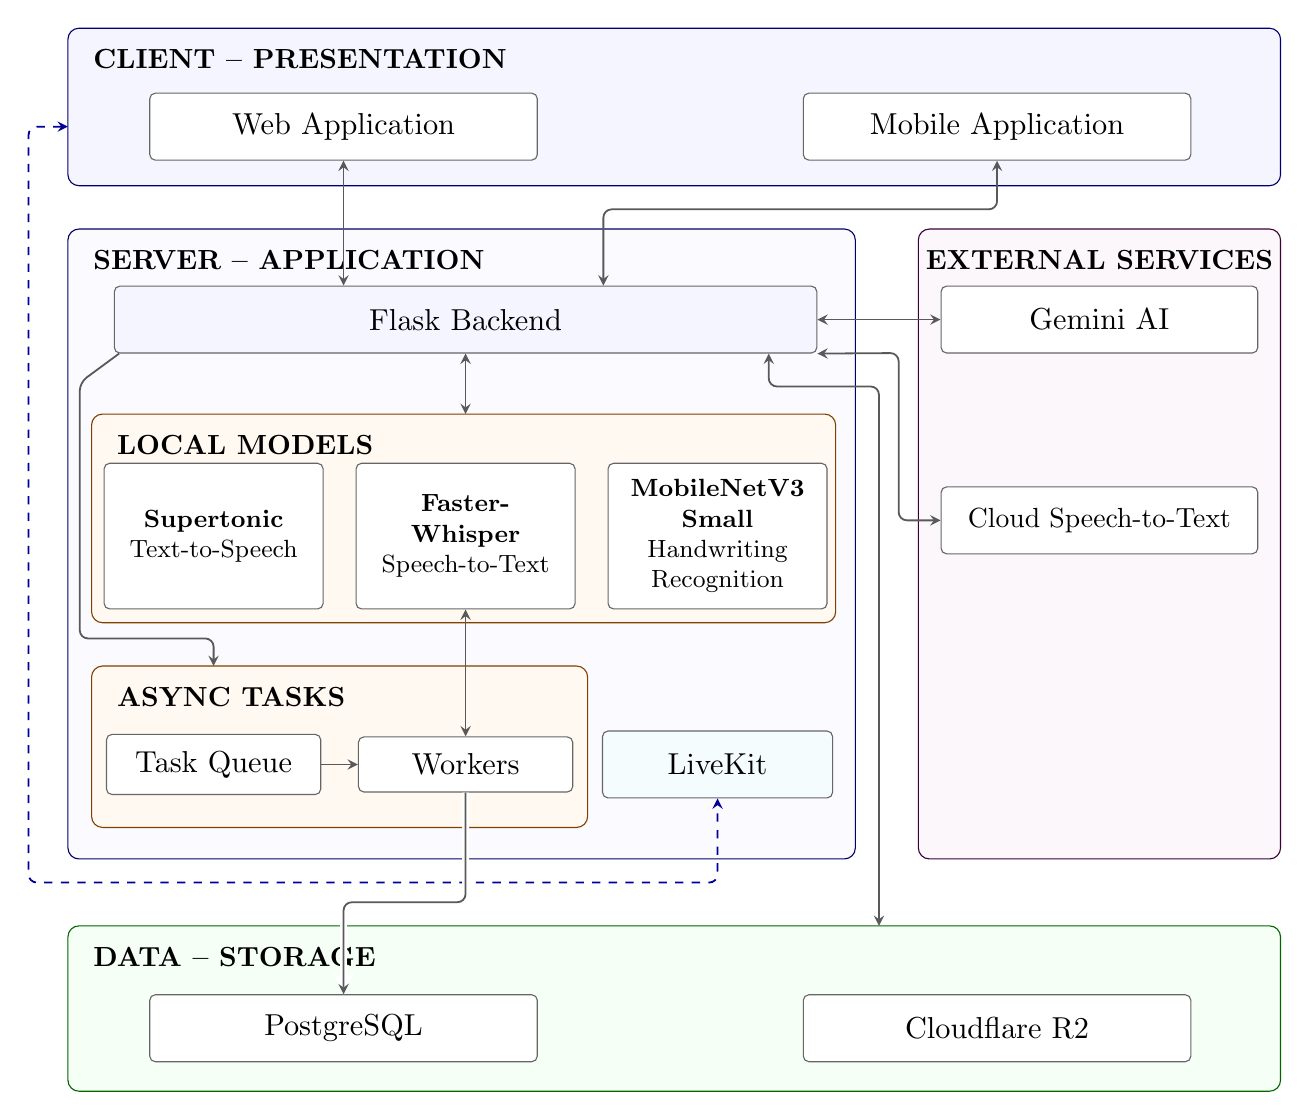
\begin{tikzpicture}[
  box/.style={draw=black!60,rounded corners=2pt,fill=white,
    text width=3.2cm,minimum height=.85cm,inner sep=6pt,
    align=center,font=\fontsize{11}{13}\selectfont},
  model/.style={box,text width=2.5cm,minimum height=1.85cm,
    font=\fontsize{9}{11}\selectfont,inner sep=4pt},
  title/.style={anchor=north west,font=\fontsize{10}{12}\selectfont\bfseries},
  link/.style={<->,>=stealth,line width=.65pt,rounded corners=3pt,draw=black!65},
  task/.style={->,>=stealth,line width=.65pt,rounded corners=3pt,draw=black!65},
  audio/.style={link,dashed,draw=blue!60!black}
]
  \draw[rounded corners,draw=blue!45!black,fill=blue!4] (-7,.9) rectangle (8.4,-1.1);
  \node[title] at (-6.8,.75) {CLIENT -- PRESENTATION};
  \node[box,text width=4.5cm] (web) at (-3.5,-.35) {Web Application};
  \node[box,text width=4.5cm] (mobile) at (4.8,-.35) {Mobile Application};

  \draw[rounded corners,draw=blue!40!black,fill=blue!2] (-7,-1.65) rectangle (3,-9.65);
  \node[title] at (-6.8,-1.8) {SERVER -- APPLICATION};
  \node[box,text width=8.5cm,fill=blue!4] (backend) at (-1.95,-2.8) {Flask Backend};
  \draw[link] (web.south) -- (web.south |- backend.north);
  \draw[link] (mobile.south) -- (4.8,-1.4) -- (-.2,-1.4) -- (-.2,0 |- backend.north);

  \draw[rounded corners,draw=orange!50!black,fill=orange!5] (-6.7,-4) rectangle (2.75,-6.65);
  \node[title] at (-6.5,-4.15) {LOCAL MODELS};
  \node[model] (tts) at (-5.15,-5.55) {\textbf{Supertonic}\\Text-to-Speech};
  \node[model] (whisper) at (-1.95,-5.55) {\textbf{Faster-Whisper}\\Speech-to-Text};
  \node[model] (kanji) at (1.25,-5.55) {\textbf{MobileNetV3}\\\textbf{Small}\\Handwriting\\Recognition};
  \draw[link] (backend.south) -- (-1.95,-4);

  \draw[rounded corners,draw=orange!50!black,fill=orange!5] (-6.7,-7.2) rectangle (-.4,-9.25);
  \node[title] at (-6.5,-7.35) {ASYNC TASKS};
  \node[box,text width=2.3cm,minimum height=.7cm] (queue) at (-5.15,-8.45) {Task Queue};
  \node[box,text width=2.3cm,minimum height=.7cm] (workers) at (-1.95,-8.45) {Workers};
  \draw[task] (queue.east) -- (workers.west);
  \draw[task] (-6.35,0 |- backend.south) -- (-6.85,-3.6) -- (-6.85,-6.85) -- (-5.15,-6.85) -- (-5.15,-7.2);
  \draw[link] (workers.north) -- (whisper.south);

  \node[box,text width=2.5cm,fill=cyan!4] (livekit) at (1.25,-8.45) {LiveKit};
  \draw[audio] (-7,-.35) -- (-7.5,-.35) -- (-7.5,-9.95) -- (1.25,-9.95) -- (livekit.south);

  \draw[rounded corners,draw=violet!45!black,fill=violet!3] (3.8,-1.65) rectangle (8.4,-9.65);
  \node[title,anchor=north] at (6.1,-1.8) {EXTERNAL SERVICES};
  \node[box,text width=3.6cm] (ai) at (6.1,-2.8) {Gemini AI};
  \node[box,text width=3.6cm,font=\fontsize{10}{12}\selectfont] (stt) at (6.1,-5.35) {Cloud Speech-to-Text};
  \draw[link] (backend.east) -- (ai.west);
  \draw[link] (backend.south east) -- (3.55,-3.225) -- (3.55,-5.35) -- (stt.west);

  \draw[rounded corners,draw=green!40!black,fill=green!4] (-7,-10.5) rectangle (8.4,-12.6);
  \node[title] at (-6.8,-10.65) {DATA -- STORAGE};
  \node[box,text width=4.5cm] (db) at (-3.5,-11.8) {PostgreSQL};
  \node[box,text width=4.5cm] (r2) at (4.8,-11.8) {Cloudflare R2};
  \draw[link] (1.9,0 |- backend.south) -- (1.9,-3.65) -- (3.3,-3.65) -- (3.3,-10.5);
  \draw[task,preaction={draw=white,line width=2.5pt}] (workers.south) -- (-1.95,-10.2) -- (-3.5,-10.2) -- (db.north);
\end{tikzpicture}
\endgroup

  \caption{Kiến trúc tổng thể hệ thống NihonGO}
  \label{fig:overall-architecture}
\end{figure}
\newpage

\clearpage
\subsection{System Components}
\subsubsection{Client Layer}
\begin{figure}[htbp]
  \centering
  \begingroup
\setstretch{1}
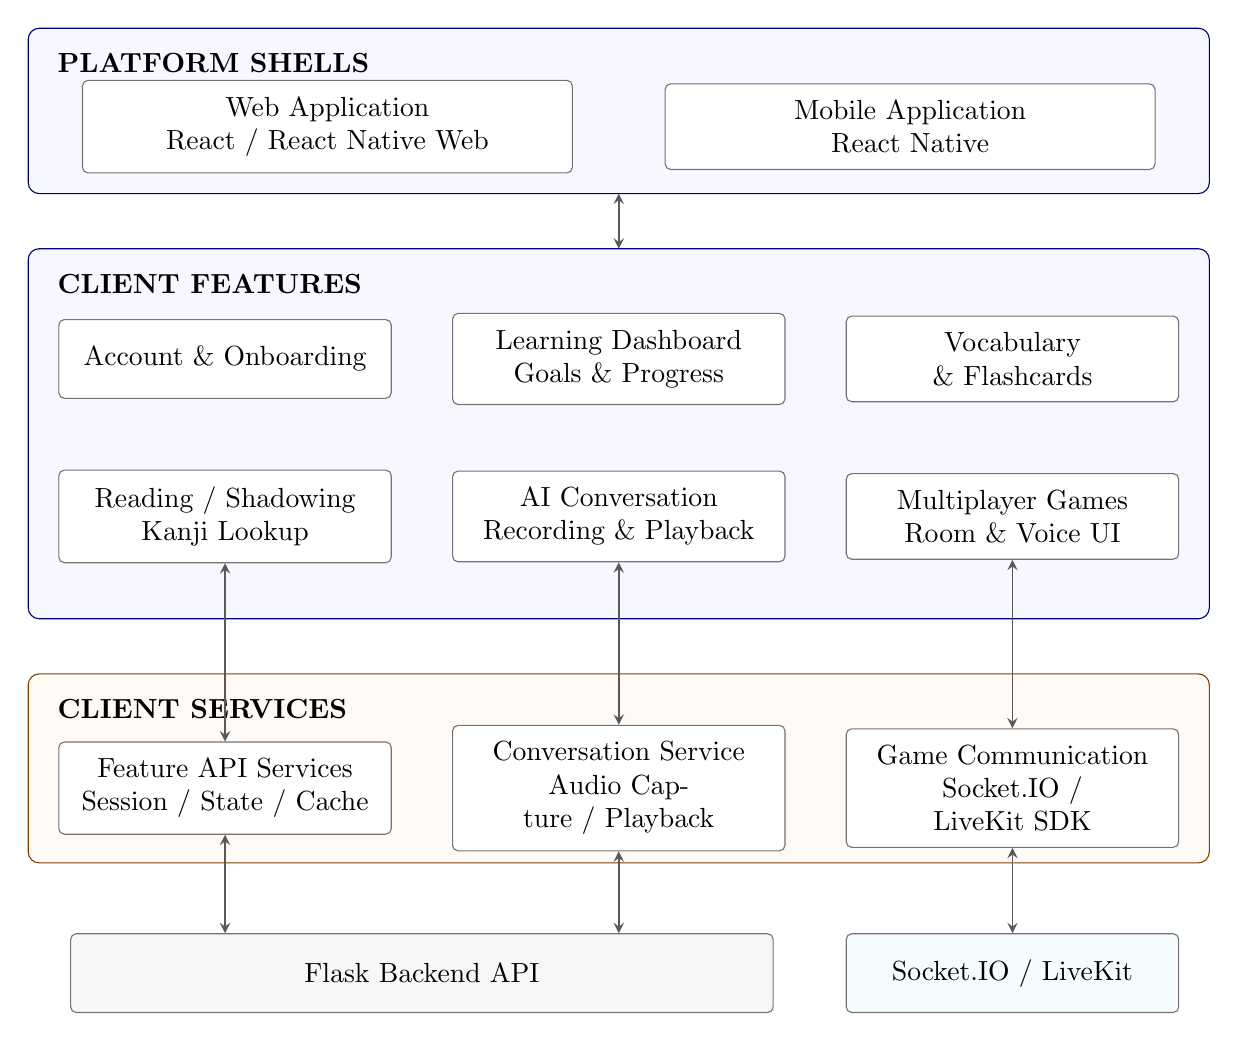
\begin{tikzpicture}[
box/.style={draw=black!55,rounded corners=2pt,fill=white,text width=3.8cm,minimum height=1cm,inner sep=6pt,align=center,font=\fontsize{10}{12}\selectfont},
title/.style={anchor=north west,font=\fontsize{10}{12}\selectfont\bfseries},
link/.style={<->,>=stealth,draw=black!65,line width=.65pt,rounded corners=3pt},
task/.style={->,>=stealth,draw=black!65,line width=.65pt,rounded corners=3pt}]

\draw[rounded corners,draw=blue!45!black,fill=blue!3] (-7.5,0) rectangle (7.5,-2.1);
\node[title] at (-7.25,-.2) {PLATFORM SHELLS};
\node[box,text width=5.8cm] at (-3.7,-1.25) {Web Application\\React / React Native Web};
\node[box,text width=5.8cm] at (3.7,-1.25) {Mobile Application\\React Native};
\draw[rounded corners,draw=blue!45!black,fill=blue!3] (-7.5,-2.8) rectangle (7.5,-7.5);
\node[title] at (-7.25,-3) {CLIENT FEATURES};
\node[box] at (-5,-4.2) {Account \& Onboarding};
\node[box] at (0,-4.2) {Learning Dashboard\\Goals \& Progress};
\node[box] at (5,-4.2) {Vocabulary \& Flashcards};
\node[box] (learning) at (-5,-6.2) {Reading / Shadowing\\Kanji Lookup};
\node[box] (speaking) at (0,-6.2) {AI Conversation\\Recording \& Playback};
\node[box] (games) at (5,-6.2) {Multiplayer Games\\Room \& Voice UI};
\draw[link] (0,-2.1) -- (0,-2.8);
\draw[rounded corners,draw=orange!50!black,fill=orange!4] (-7.5,-8.2) rectangle (7.5,-10.6);
\node[title] at (-7.25,-8.4) {CLIENT SERVICES};
\node[box] (api) at (-5,-9.65) {Feature API Services\\Session / State / Cache};
\node[box] (voice) at (0,-9.65) {Conversation Service\\Audio Capture / Playback};
\node[box] (realtime) at (5,-9.65) {Game Communication\\Socket.IO / LiveKit SDK};
\draw[link] (learning.south) -- (api.north);
\draw[link] (speaking.south) -- (voice.north);
\draw[link] (games.south) -- (realtime.north);
\node[box,text width=8.5cm,fill=black!3] (server) at (-2.5,-12) {Flask Backend API};
\node[box,fill=cyan!4] (media) at (5,-12) {Socket.IO / LiveKit};
\draw[link] (api.south) -- (-5,0 |- server.north);
\draw[link] (voice.south) -- (0,0 |- server.north);
\draw[link] (realtime.south) -- (media.north);
\end{tikzpicture}
\endgroup

  \caption{Kiến trúc chi tiết tầng Client}
  \label{fig:client-layer}
\end{figure}
\clearpage
\subsubsection{Application Layer}
\begin{figure}[htbp]
  \centering
  \begingroup
\setstretch{1}
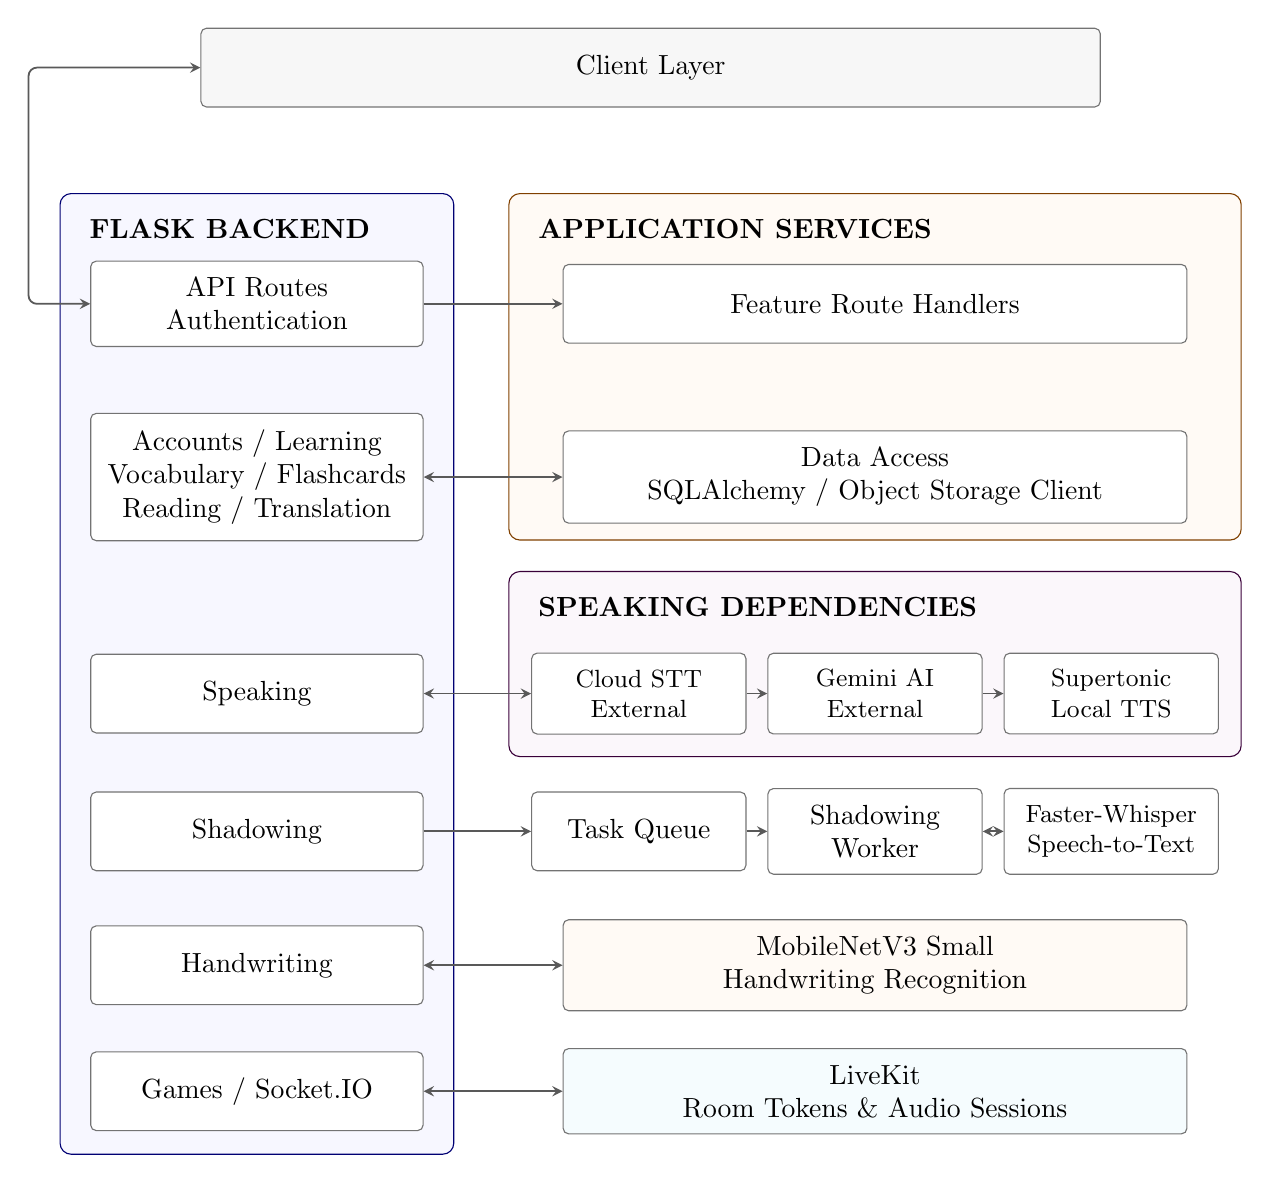
\begin{tikzpicture}[
box/.style={draw=black!55,rounded corners=2pt,fill=white,text width=3.8cm,minimum height=1cm,inner sep=6pt,align=center,font=\fontsize{10}{12}\selectfont},
title/.style={anchor=north west,font=\fontsize{10}{12}\selectfont\bfseries},
link/.style={<->,>=stealth,draw=black!65,line width=.65pt,rounded corners=3pt},
task/.style={->,>=stealth,draw=black!65,line width=.65pt,rounded corners=3pt}]

\node[box,text width=11cm,fill=black!3] (client) at (0,0) {Client Layer};
\draw[rounded corners,draw=blue!45!black,fill=blue!3] (-7.5,-1.6) rectangle (-2.5,-13.8);
\node[title] at (-7.25,-1.8) {FLASK BACKEND};
\node[box] (api) at (-5,-3) {API Routes\\Authentication};
\node[box] (core) at (-5,-5.2) {Accounts / Learning\\Vocabulary / Flashcards\\Reading / Translation};
\node[box] (speaking) at (-5,-7.95) {Speaking};
\node[box] (shadow) at (-5,-9.7) {Shadowing};
\node[box] (hand) at (-5,-11.4) {Handwriting};
\node[box] (games) at (-5,-13) {Games / Socket.IO};
\draw[link] (client.west) -- (-7.9,0) -- (-7.9,-3) -- (api.west);
\draw[rounded corners,draw=orange!50!black,fill=orange!4] (-1.8,-1.6) rectangle (7.5,-6);
\node[title] at (-1.55,-1.8) {APPLICATION SERVICES};
\node[box,text width=7.5cm] (handlers) at (2.85,-3) {Feature Route Handlers};
\node[box,text width=7.5cm] (data) at (2.85,-5.2) {Data Access\\SQLAlchemy / Object Storage Client};
\draw[task] (api.east) -- (handlers.west);
\draw[link] (core.east) -- (data.west);
\draw[rounded corners,draw=violet!45!black,fill=violet!3] (-1.8,-6.4) rectangle (7.5,-8.75);
\node[title] at (-1.55,-6.6) {SPEAKING DEPENDENCIES};
\node[box,text width=2.3cm,font=\fontsize{9}{11}\selectfont] (stt) at (-.15,-7.95) {Cloud STT\\External};
\node[box,text width=2.3cm,font=\fontsize{9}{11}\selectfont] (ai) at (2.85,-7.95) {Gemini AI\\External};
\node[box,text width=2.3cm,font=\fontsize{9}{11}\selectfont] (tts) at (5.85,-7.95) {Supertonic\\Local TTS};
\draw[link] (speaking.east) -- (stt.west);
\draw[task] (stt.east) -- (ai.west);
\draw[task] (ai.east) -- (tts.west);
\node[box,text width=2.3cm] (q) at (-.15,-9.7) {Task Queue};
\node[box,text width=2.3cm] (w) at (2.85,-9.7) {Shadowing Worker};
\node[box,text width=2.3cm,font=\fontsize{9}{11}\selectfont] (whisper) at (5.85,-9.7) {Faster-Whisper\\Speech-to-Text};
\draw[task] (shadow.east) -- (q.west);
\draw[task] (q.east) -- (w.west);
\draw[link] (w.east) -- (whisper.west);
\node[box,text width=7.5cm,fill=orange!4] (model) at (2.85,-11.4) {MobileNetV3 Small\\Handwriting Recognition};
\draw[link] (hand.east) -- (model.west);
\node[box,text width=7.5cm,fill=cyan!4] (live) at (2.85,-13) {LiveKit\\Room Tokens \& Audio Sessions};
\draw[link] (games.east) -- (live.west);
\end{tikzpicture}
\endgroup

  \caption{Kiến trúc chi tiết tầng Application}
  \label{fig:application-layer}
\end{figure}
\clearpage
\subsubsection{Data Layer}
\begin{figure}[htbp]
  \centering
  \begingroup
\setstretch{1}
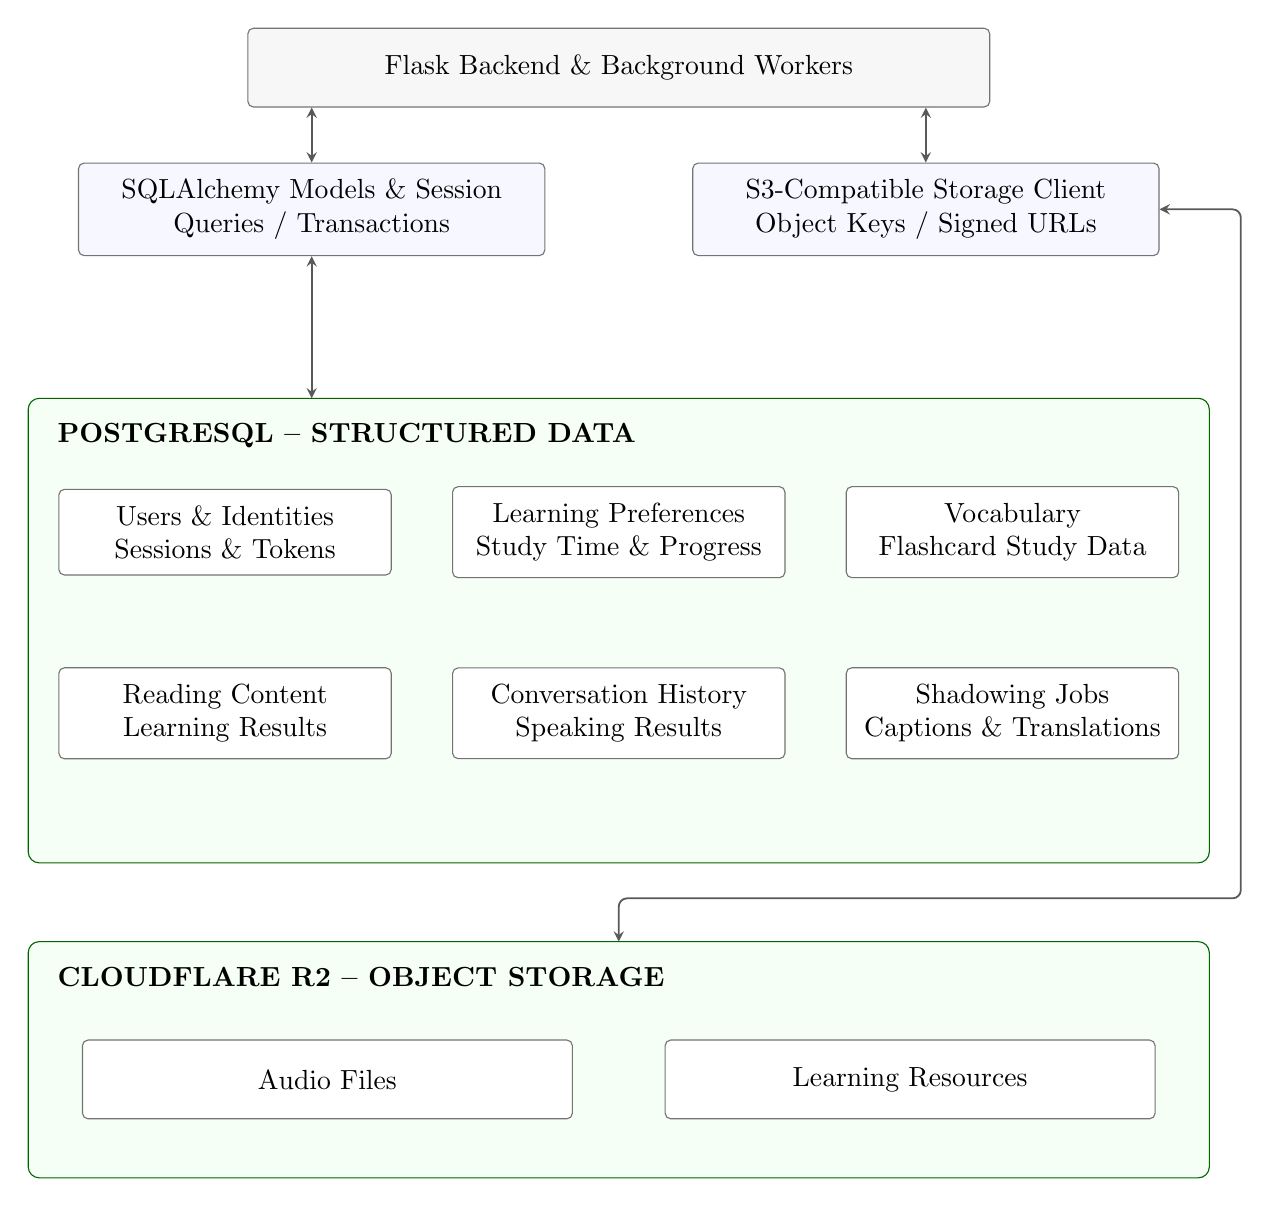
\begin{tikzpicture}[
box/.style={draw=black!55,rounded corners=2pt,fill=white,text width=3.8cm,minimum height=1cm,inner sep=6pt,align=center,font=\fontsize{10}{12}\selectfont},
title/.style={anchor=north west,font=\fontsize{10}{12}\selectfont\bfseries},
link/.style={<->,>=stealth,draw=black!65,line width=.65pt,rounded corners=3pt},
task/.style={->,>=stealth,draw=black!65,line width=.65pt,rounded corners=3pt}]

\node[box,text width=9cm,fill=black!3] (app) at (0,0) {Flask Backend \& Background Workers};
\node[box,text width=5.5cm,fill=blue!3] (orm) at (-3.9,-1.8) {SQLAlchemy Models \& Session\\Queries / Transactions};
\node[box,text width=5.5cm,fill=blue!3] (storage) at (3.9,-1.8) {S3-Compatible Storage Client\\Object Keys / Signed URLs};
\draw[link] (-3.9,0 |- app.south) -- (orm.north);
\draw[link] (3.9,0 |- app.south) -- (storage.north);
\begin{scope}[yshift=-2.6cm]
\draw[rounded corners,draw=green!40!black,fill=green!4] (-7.5,-1.6) rectangle (7.5,-7.5);
\node[title] at (-7.25,-1.8) {POSTGRESQL -- STRUCTURED DATA};
\node[box] at (-5,-3.3) {Users \& Identities\\Sessions \& Tokens};
\node[box] at (0,-3.3) {Learning Preferences\\Study Time \& Progress};
\node[box] at (5,-3.3) {Vocabulary\\Flashcard Study Data};
\node[box] at (-5,-5.6) {Reading Content\\Learning Results};
\node[box] at (0,-5.6) {Conversation History\\Speaking Results};
\node[box] at (5,-5.6) {Shadowing Jobs\\Captions \& Translations};
\draw[rounded corners,draw=green!40!black,fill=green!4] (-7.5,-8.5) rectangle (7.5,-11.5);
\node[title] at (-7.25,-8.7) {CLOUDFLARE R2 -- OBJECT STORAGE};
\node[box,text width=5.8cm] at (-3.7,-10.25) {Audio Files};
\node[box,text width=5.8cm] at (3.7,-10.25) {Learning Resources};
\end{scope}
\draw[link] (orm.south) -- (-3.9,-4.2);
\draw[link] (storage.east) -- (7.9,-1.8) -- (7.9,-10.55) -- (0,-10.55) -- (0,-11.1);
\end{tikzpicture}
\endgroup

  \caption{Kiến trúc chi tiết tầng Data}
  \label{fig:data-layer}
\end{figure}
\clearpage
\section{DATABASE DESIGN}
\subsection{Database Overview}
Các sơ đồ mô tả 54 bảng từ các model SQLAlchemy, được đối chiếu với migrations của backend. Sơ đồ tổng quan chọn các bảng trung tâm; các hình chi tiết chia theo nhóm nghiệp vụ và có thể lặp lại bảng tham chiếu.

\noindent{\small\raggedright\textbf{Quy ước:} PK là khóa chính, FK là khóa ngoại; nhiều trường cùng mang PK tạo khóa chính ghép. Dấu ? chỉ trường cho phép NULL. Nhãn 1, 0..1 và 0..N biểu diễn số bản ghi ở mỗi đầu quan hệ. Mỗi khối chỉ liệt kê các trường khóa và một số thuộc tính chính; các đường nối biểu diễn FK thực tế. Bảng không có FK được giữ độc lập.\par}

\begin{figure}[htbp]
  \centering
  \begingroup
\setstretch{1}
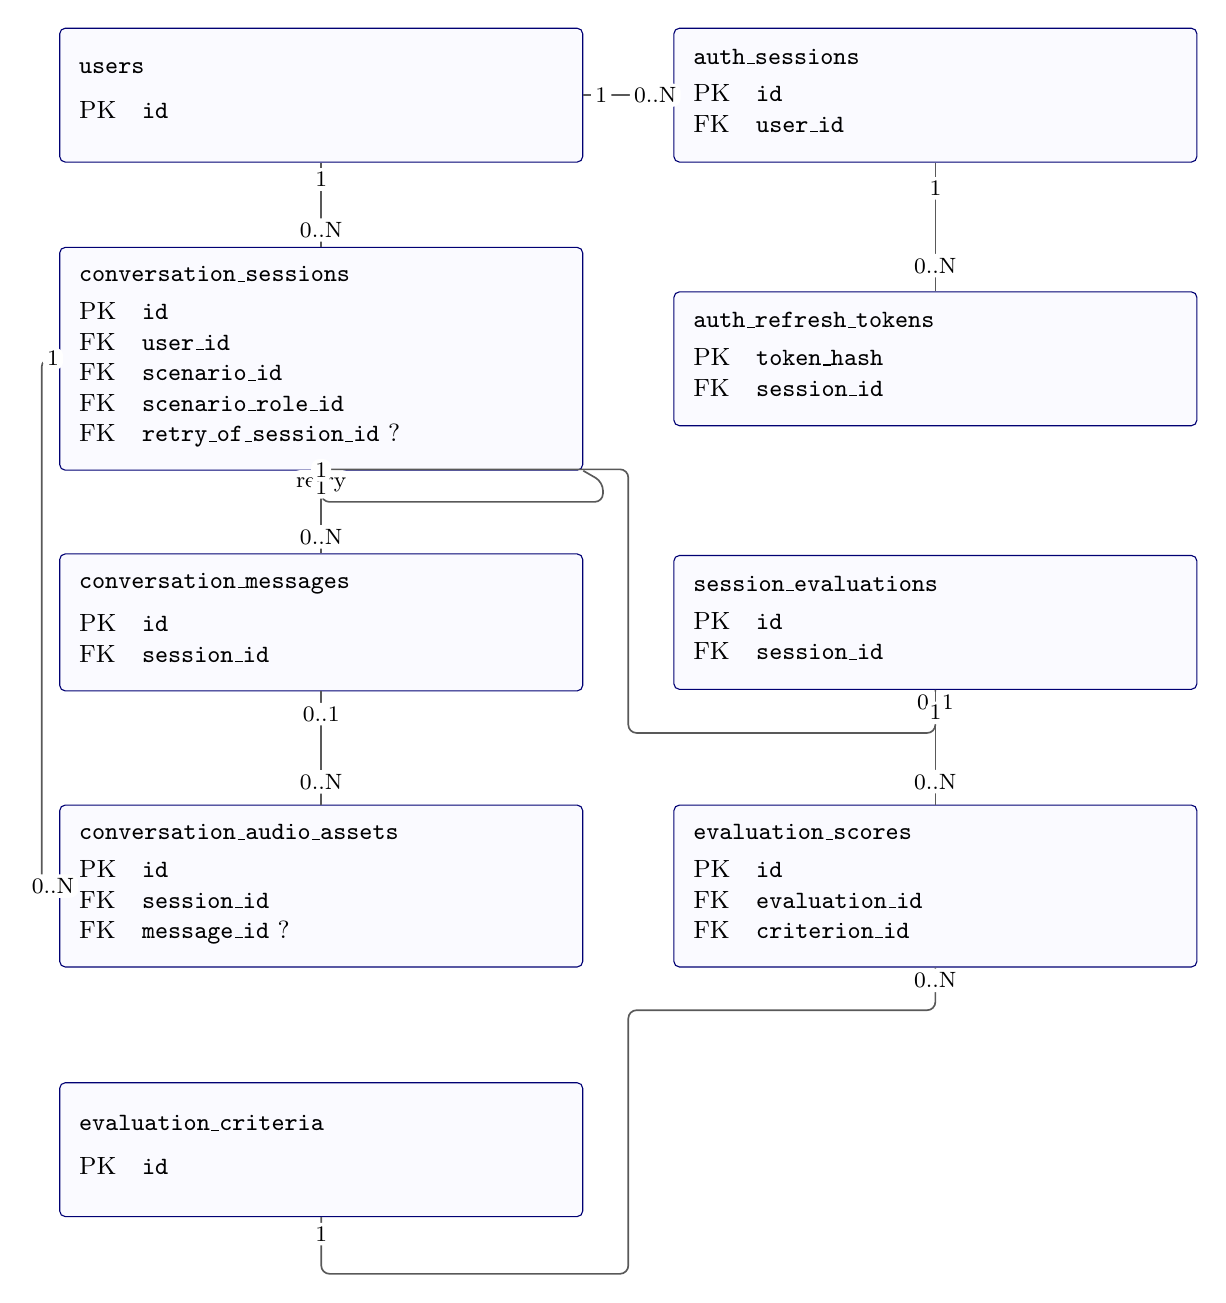
\begin{tikzpicture}[
entity/.style={draw=blue!45!black,rounded corners=2pt,fill=blue!2,inner sep=7pt,text width=6.15cm,minimum height=3.3cm,align=left,font=\fontsize{9}{11}\selectfont},
rel/.style={draw=black!65,line width=.6pt,rounded corners=3pt},
card/.style={fill=white,inner sep=1.5pt,font=\fontsize{8}{9}\selectfont}]
\node[entity,minimum height=1.7cm] (users) at (-3.9,0) {\textbf{\texttt{users}}\\[5pt]\begin{tabular}{@{}l@{\quad}l@{}}PK & \texttt{id} \\\end{tabular}};
\node[entity,minimum height=1.7cm] (authsessions) at (3.9,0) {\textbf{\texttt{auth\_sessions}}\\[5pt]\begin{tabular}{@{}l@{\quad}l@{}}PK & \texttt{id} \\
FK & \texttt{user\_id} \\\end{tabular}};
\node[entity,minimum height=1.7cm] (conversationsessions) at (-3.9,-3.348) {\textbf{\texttt{conversation\_sessions}}\\[5pt]\begin{tabular}{@{}l@{\quad}l@{}}PK & \texttt{id} \\
FK & \texttt{user\_id} \\
FK & \texttt{scenario\_id} \\
FK & \texttt{scenario\_role\_id} \\
FK & \texttt{retry\_of\_session\_id} ? \\\end{tabular}};
\node[entity,minimum height=1.7cm] (authrefreshtokens) at (3.9,-3.348) {\textbf{\texttt{auth\_refresh\_tokens}}\\[5pt]\begin{tabular}{@{}l@{\quad}l@{}}PK & \texttt{token\_hash} \\
FK & \texttt{session\_id} \\\end{tabular}};
\node[entity,minimum height=1.7cm] (conversationmessages) at (-3.9,-6.696) {\textbf{\texttt{conversation\_messages}}\\[5pt]\begin{tabular}{@{}l@{\quad}l@{}}PK & \texttt{id} \\
FK & \texttt{session\_id} \\\end{tabular}};
\node[entity,minimum height=1.7cm] (sessionevaluations) at (3.9,-6.696) {\textbf{\texttt{session\_evaluations}}\\[5pt]\begin{tabular}{@{}l@{\quad}l@{}}PK & \texttt{id} \\
FK & \texttt{session\_id} \\\end{tabular}};
\node[entity,minimum height=1.7cm] (conversationaudioassets) at (-3.9,-10.044) {\textbf{\texttt{conversation\_audio\_assets}}\\[5pt]\begin{tabular}{@{}l@{\quad}l@{}}PK & \texttt{id} \\
FK & \texttt{session\_id} \\
FK & \texttt{message\_id} ? \\\end{tabular}};
\node[entity,minimum height=1.7cm] (evaluationscores) at (3.9,-10.044) {\textbf{\texttt{evaluation\_scores}}\\[5pt]\begin{tabular}{@{}l@{\quad}l@{}}PK & \texttt{id} \\
FK & \texttt{evaluation\_id} \\
FK & \texttt{criterion\_id} \\\end{tabular}};
\node[entity,minimum height=1.7cm] (evaluationcriteria) at (-3.9,-13.392) {\textbf{\texttt{evaluation\_criteria}}\\[5pt]\begin{tabular}{@{}l@{\quad}l@{}}PK & \texttt{id} \\\end{tabular}};
\draw[rel] (authsessions.west) -- node[card,pos=.2]{0..N} node[card,pos=.8]{1} (users.east);
\draw[rel] (conversationsessions.north) -- node[card,pos=.2]{0..N} node[card,pos=.8]{1} (users.south);
\draw[rel] (conversationsessions.south east) -- ++(.25,-0.144) -- ++(0,-0.252) -| (conversationsessions.south) node[card,pos=.8]{retry};
\draw[rel] (authrefreshtokens.north) -- node[card,pos=.2]{0..N} node[card,pos=.8]{1} (authsessions.south);
\draw[rel] (conversationmessages.north) -- node[card,pos=.2]{0..N} node[card,pos=.8]{1} (conversationsessions.south);
\draw[rel] (sessionevaluations.south) -- node[card,pos=.3]{0..1} (3.9,-8.1) -- (0,-8.1) -- (0,-4.752) -- (-3.9,-4.752) -- node[card,pos=.7]{1} (conversationsessions.south);
\draw[rel] (conversationaudioassets.north) -- node[card,pos=.2]{0..N} node[card,pos=.8]{0..1} (conversationmessages.south);
\draw[rel] (conversationaudioassets.west) -- node[card,pos=.35]{0..N} (-7.449999999999999,-10.044) -- (-7.449999999999999,-3.348) -- node[card,pos=.65]{1} (conversationsessions.west);
\draw[rel] (evaluationscores.south) -- node[card,pos=.3]{0..N} (3.9,-11.621) -- (0,-11.621) -- (0,-14.969) -- (-3.9,-14.969) -- node[card,pos=.7]{1} (evaluationcriteria.south);
\draw[rel] (evaluationscores.north) -- node[card,pos=.2]{0..N} node[card,pos=.8]{1} (sessionevaluations.south);
\end{tikzpicture}
\endgroup

  \caption{ERD tổng quan các bảng trung tâm}
  \label{fig:erd-overview}
\end{figure}
\clearpage
\subsection{Accounts and Authentication}
\begin{figure}[htbp]
  \centering
  \begingroup
\setstretch{1}
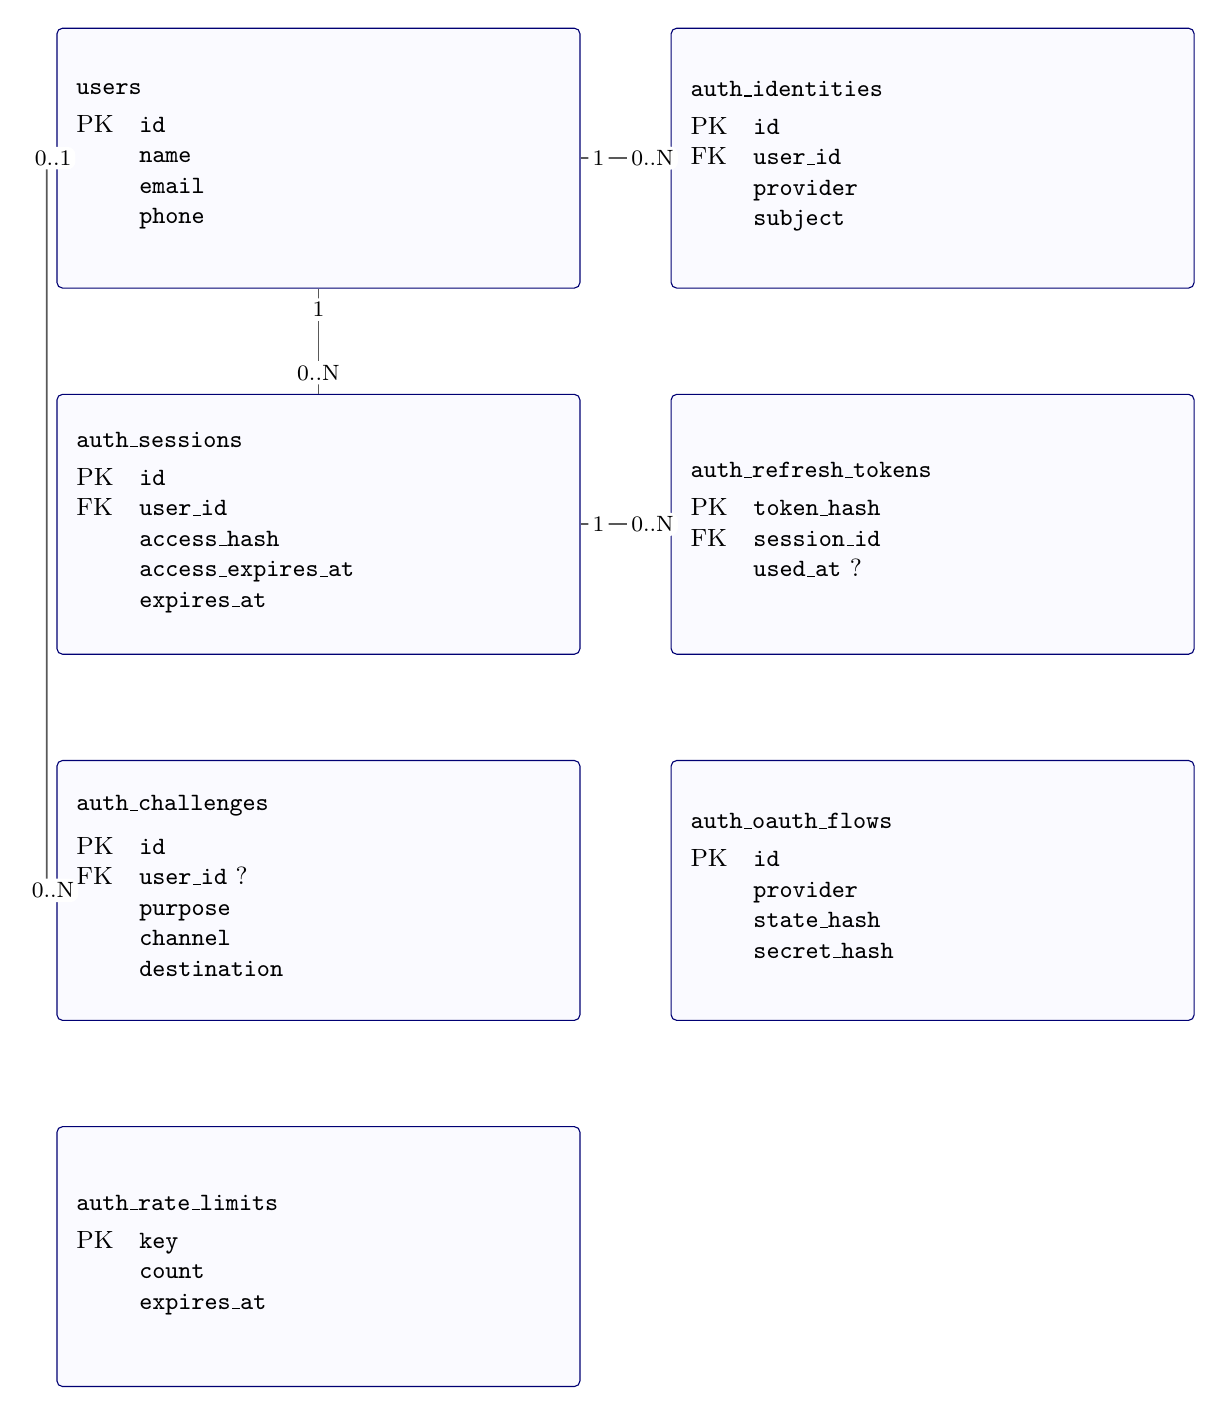
\begin{tikzpicture}[
entity/.style={draw=blue!45!black,rounded corners=2pt,fill=blue!2,inner sep=7pt,text width=6.15cm,minimum height=3.3cm,align=left,font=\fontsize{9}{11}\selectfont},
rel/.style={draw=black!65,line width=.6pt,rounded corners=3pt},
card/.style={fill=white,inner sep=1.5pt,font=\fontsize{8}{9}\selectfont}]
\node[entity] (users) at (-3.9,0) {\textbf{\texttt{users}}\\[5pt]\begin{tabular}{@{}l@{\quad}l@{}}PK & \texttt{id} \\
 & \texttt{name} \\
 & \texttt{email} \\
 & \texttt{phone} \\\end{tabular}};
\node[entity] (authidentities) at (3.9,0) {\textbf{\texttt{auth\_identities}}\\[5pt]\begin{tabular}{@{}l@{\quad}l@{}}PK & \texttt{id} \\
FK & \texttt{user\_id} \\
 & \texttt{provider} \\
 & \texttt{subject} \\\end{tabular}};
\node[entity] (authsessions) at (-3.9,-4.65) {\textbf{\texttt{auth\_sessions}}\\[5pt]\begin{tabular}{@{}l@{\quad}l@{}}PK & \texttt{id} \\
FK & \texttt{user\_id} \\
 & \texttt{access\_hash} \\
 & \texttt{access\_expires\_at} \\
 & \texttt{expires\_at} \\\end{tabular}};
\node[entity] (authrefreshtokens) at (3.9,-4.65) {\textbf{\texttt{auth\_refresh\_tokens}}\\[5pt]\begin{tabular}{@{}l@{\quad}l@{}}PK & \texttt{token\_hash} \\
FK & \texttt{session\_id} \\
 & \texttt{used\_at} ? \\\end{tabular}};
\node[entity] (authchallenges) at (-3.9,-9.3) {\textbf{\texttt{auth\_challenges}}\\[5pt]\begin{tabular}{@{}l@{\quad}l@{}}PK & \texttt{id} \\
FK & \texttt{user\_id} ? \\
 & \texttt{purpose} \\
 & \texttt{channel} \\
 & \texttt{destination} \\\end{tabular}};
\node[entity] (authoauthflows) at (3.9,-9.3) {\textbf{\texttt{auth\_oauth\_flows}}\\[5pt]\begin{tabular}{@{}l@{\quad}l@{}}PK & \texttt{id} \\
 & \texttt{provider} \\
 & \texttt{state\_hash} \\
 & \texttt{secret\_hash} \\\end{tabular}};
\node[entity] (authratelimits) at (-3.9,-13.950000000000001) {\textbf{\texttt{auth\_rate\_limits}}\\[5pt]\begin{tabular}{@{}l@{\quad}l@{}}PK & \texttt{key} \\
 & \texttt{count} \\
 & \texttt{expires\_at} \\\end{tabular}};
\draw[rel] (authidentities.west) -- node[card,pos=.2]{0..N} node[card,pos=.8]{1} (users.east);
\draw[rel] (authsessions.north) -- node[card,pos=.2]{0..N} node[card,pos=.8]{1} (users.south);
\draw[rel] (authrefreshtokens.west) -- node[card,pos=.2]{0..N} node[card,pos=.8]{1} (authsessions.east);
\draw[rel] (authchallenges.west) -- node[card,pos=.35]{0..N} (-7.35,-9.3) -- (-7.35,0) -- node[card,pos=.65]{0..1} (users.west);
\end{tikzpicture}
\endgroup

  \caption{ERD: Accounts and Authentication}
  \label{fig:erd-auth}
\end{figure}
\clearpage
\subsection{Learning and Flashcard Collections}
\begin{figure}[htbp]
  \centering
  \begingroup
\setstretch{1}
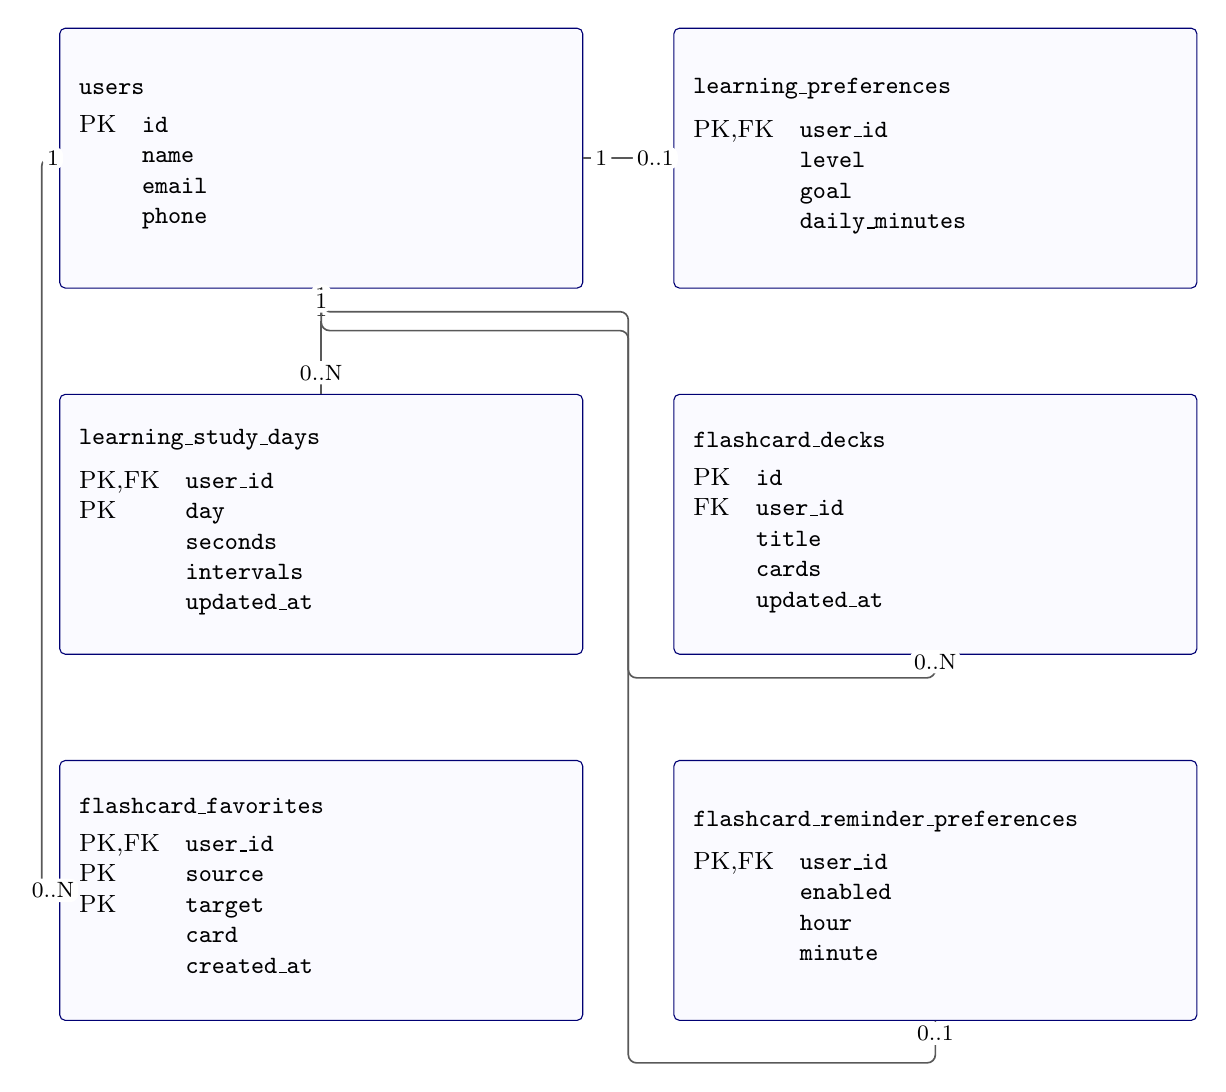
\begin{tikzpicture}[
entity/.style={draw=blue!45!black,rounded corners=2pt,fill=blue!2,inner sep=7pt,text width=6.15cm,minimum height=3.3cm,align=left,font=\fontsize{9}{11}\selectfont},
rel/.style={draw=black!65,line width=.6pt,rounded corners=3pt},
card/.style={fill=white,inner sep=1.5pt,font=\fontsize{8}{9}\selectfont}]
\node[entity] (users) at (-3.9,0) {\textbf{\texttt{users}}\\[5pt]\begin{tabular}{@{}l@{\quad}l@{}}PK & \texttt{id} \\
 & \texttt{name} \\
 & \texttt{email} \\
 & \texttt{phone} \\\end{tabular}};
\node[entity] (learningpreferences) at (3.9,0) {\textbf{\texttt{learning\_preferences}}\\[5pt]\begin{tabular}{@{}l@{\quad}l@{}}PK,FK & \texttt{user\_id} \\
 & \texttt{level} \\
 & \texttt{goal} \\
 & \texttt{daily\_minutes} \\\end{tabular}};
\node[entity] (learningstudydays) at (-3.9,-4.65) {\textbf{\texttt{learning\_study\_days}}\\[5pt]\begin{tabular}{@{}l@{\quad}l@{}}PK,FK & \texttt{user\_id} \\
PK & \texttt{day} \\
 & \texttt{seconds} \\
 & \texttt{intervals} \\
 & \texttt{updated\_at} \\\end{tabular}};
\node[entity] (flashcarddecks) at (3.9,-4.65) {\textbf{\texttt{flashcard\_decks}}\\[5pt]\begin{tabular}{@{}l@{\quad}l@{}}PK & \texttt{id} \\
FK & \texttt{user\_id} \\
 & \texttt{title} \\
 & \texttt{cards} \\
 & \texttt{updated\_at} \\\end{tabular}};
\node[entity] (flashcardfavorites) at (-3.9,-9.3) {\textbf{\texttt{flashcard\_favorites}}\\[5pt]\begin{tabular}{@{}l@{\quad}l@{}}PK,FK & \texttt{user\_id} \\
PK & \texttt{source} \\
PK & \texttt{target} \\
 & \texttt{card} \\
 & \texttt{created\_at} \\\end{tabular}};
\node[entity] (flashcardreminderpreferences) at (3.9,-9.3) {\textbf{\texttt{flashcard\_reminder\_preferences}}\\[5pt]\begin{tabular}{@{}l@{\quad}l@{}}PK,FK & \texttt{user\_id} \\
 & \texttt{enabled} \\
 & \texttt{hour} \\
 & \texttt{minute} \\\end{tabular}};
\draw[rel] (learningpreferences.west) -- node[card,pos=.2]{0..1} node[card,pos=.8]{1} (users.east);
\draw[rel] (learningstudydays.north) -- node[card,pos=.2]{0..N} node[card,pos=.8]{1} (users.south);
\draw[rel] (flashcarddecks.south) -- node[card,pos=.3]{0..N} (3.9,-6.6000000000000005) -- (0,-6.6000000000000005) -- (0,-1.95) -- (-3.9,-1.95) -- node[card,pos=.7]{1} (users.south);
\draw[rel] (flashcardfavorites.west) -- node[card,pos=.35]{0..N} (-7.449999999999999,-9.3) -- (-7.449999999999999,0) -- node[card,pos=.65]{1} (users.west);
\draw[rel] (flashcardreminderpreferences.south) -- node[card,pos=.3]{0..1} (3.9,-11.49) -- (0,-11.49) -- (0,-2.19) -- (-3.9,-2.19) -- node[card,pos=.7]{1} (users.south);
\end{tikzpicture}
\endgroup

  \caption{ERD: Learning and Flashcard Collections}
  \label{fig:erd-learning}
\end{figure}
\clearpage
\subsection{Flashcard Sessions and Reviews}
{\small\raggedright Các trường \texttt{deck\_id} và \texttt{card\_id} không được khai báo FK; vì vậy hình không nối chúng với bảng deck hoặc bảng từ vựng.\par}

\begin{figure}[htbp]
  \centering
  \begingroup
\setstretch{1}
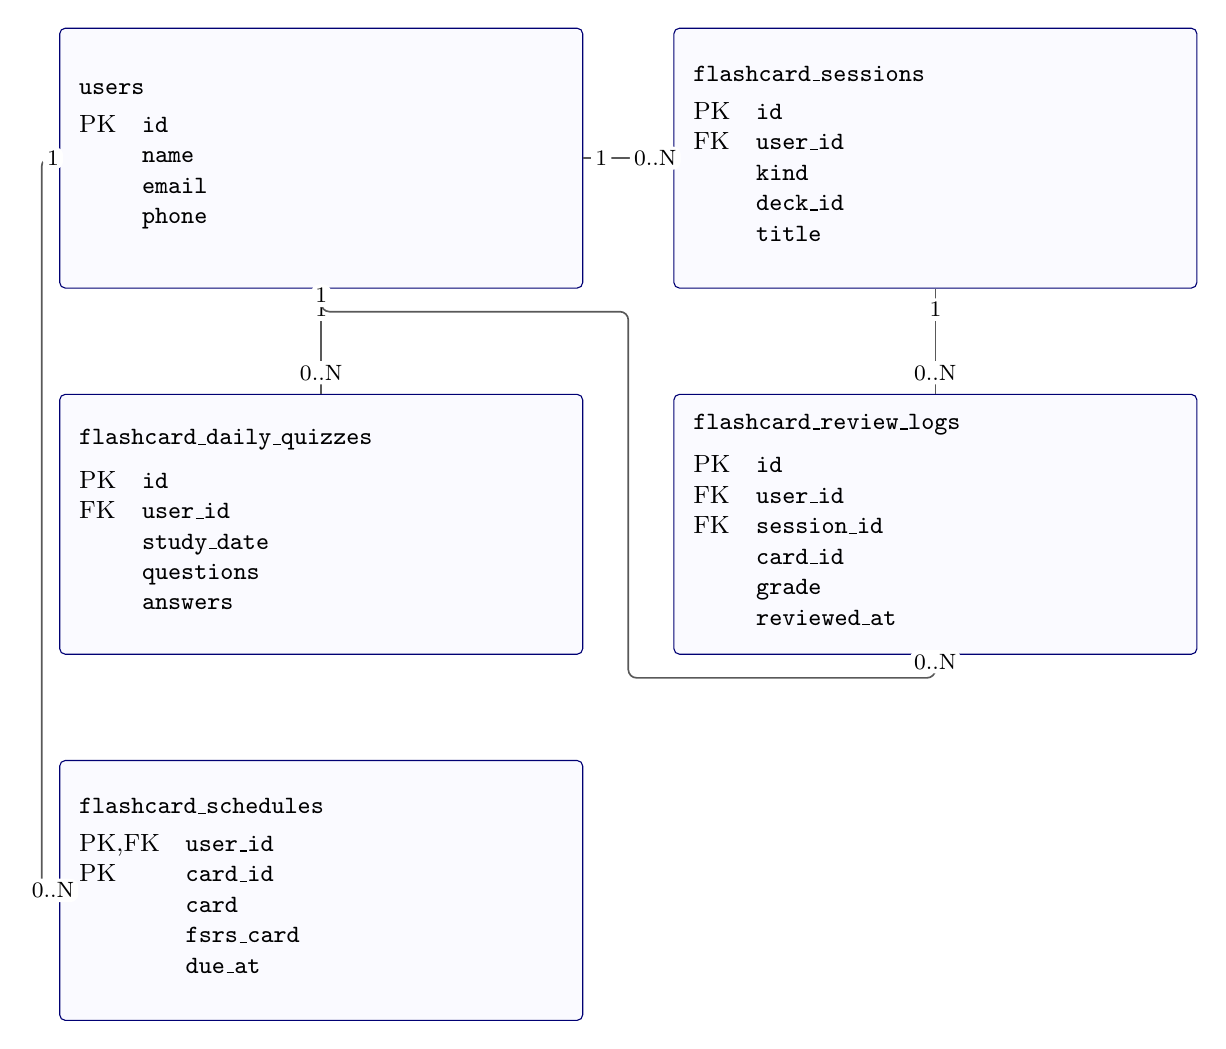
\begin{tikzpicture}[
entity/.style={draw=blue!45!black,rounded corners=2pt,fill=blue!2,inner sep=7pt,text width=6.15cm,minimum height=3.3cm,align=left,font=\fontsize{9}{11}\selectfont},
rel/.style={draw=black!65,line width=.6pt,rounded corners=3pt},
card/.style={fill=white,inner sep=1.5pt,font=\fontsize{8}{9}\selectfont}]
\node[entity] (users) at (-3.9,0) {\textbf{\texttt{users}}\\[5pt]\begin{tabular}{@{}l@{\quad}l@{}}PK & \texttt{id} \\
 & \texttt{name} \\
 & \texttt{email} \\
 & \texttt{phone} \\\end{tabular}};
\node[entity] (flashcardsessions) at (3.9,0) {\textbf{\texttt{flashcard\_sessions}}\\[5pt]\begin{tabular}{@{}l@{\quad}l@{}}PK & \texttt{id} \\
FK & \texttt{user\_id} \\
 & \texttt{kind} \\
 & \texttt{deck\_id} \\
 & \texttt{title} \\\end{tabular}};
\node[entity] (flashcarddailyquizzes) at (-3.9,-4.65) {\textbf{\texttt{flashcard\_daily\_quizzes}}\\[5pt]\begin{tabular}{@{}l@{\quad}l@{}}PK & \texttt{id} \\
FK & \texttt{user\_id} \\
 & \texttt{study\_date} \\
 & \texttt{questions} \\
 & \texttt{answers} \\\end{tabular}};
\node[entity] (flashcardreviewlogs) at (3.9,-4.65) {\textbf{\texttt{flashcard\_review\_logs}}\\[5pt]\begin{tabular}{@{}l@{\quad}l@{}}PK & \texttt{id} \\
FK & \texttt{user\_id} \\
FK & \texttt{session\_id} \\
 & \texttt{card\_id} \\
 & \texttt{grade} \\
 & \texttt{reviewed\_at} \\\end{tabular}};
\node[entity] (flashcardschedules) at (-3.9,-9.3) {\textbf{\texttt{flashcard\_schedules}}\\[5pt]\begin{tabular}{@{}l@{\quad}l@{}}PK,FK & \texttt{user\_id} \\
PK & \texttt{card\_id} \\
 & \texttt{card} \\
 & \texttt{fsrs\_card} \\
 & \texttt{due\_at} \\\end{tabular}};
\draw[rel] (flashcardsessions.west) -- node[card,pos=.2]{0..N} node[card,pos=.8]{1} (users.east);
\draw[rel] (flashcarddailyquizzes.north) -- node[card,pos=.2]{0..N} node[card,pos=.8]{1} (users.south);
\draw[rel] (flashcardreviewlogs.south) -- node[card,pos=.3]{0..N} (3.9,-6.6000000000000005) -- (0,-6.6000000000000005) -- (0,-1.95) -- (-3.9,-1.95) -- node[card,pos=.7]{1} (users.south);
\draw[rel] (flashcardreviewlogs.north) -- node[card,pos=.2]{0..N} node[card,pos=.8]{1} (flashcardsessions.south);
\draw[rel] (flashcardschedules.west) -- node[card,pos=.35]{0..N} (-7.449999999999999,-9.3) -- (-7.449999999999999,0) -- node[card,pos=.65]{1} (users.west);
\end{tikzpicture}
\endgroup

  \caption{ERD: Flashcard Sessions and Reviews}
  \label{fig:erd-reviews}
\end{figure}
\clearpage
\subsection{Vocabulary and Dictionary}
{\small\raggedright Trường \texttt{dictionary\_history.user\_id} tham chiếu \texttt{users.id} ở nhóm tài khoản. Không có FK từ các bảng từ điển sang bảng từ vựng.\par}

\begin{figure}[htbp]
  \centering
  \begingroup
\setstretch{1}
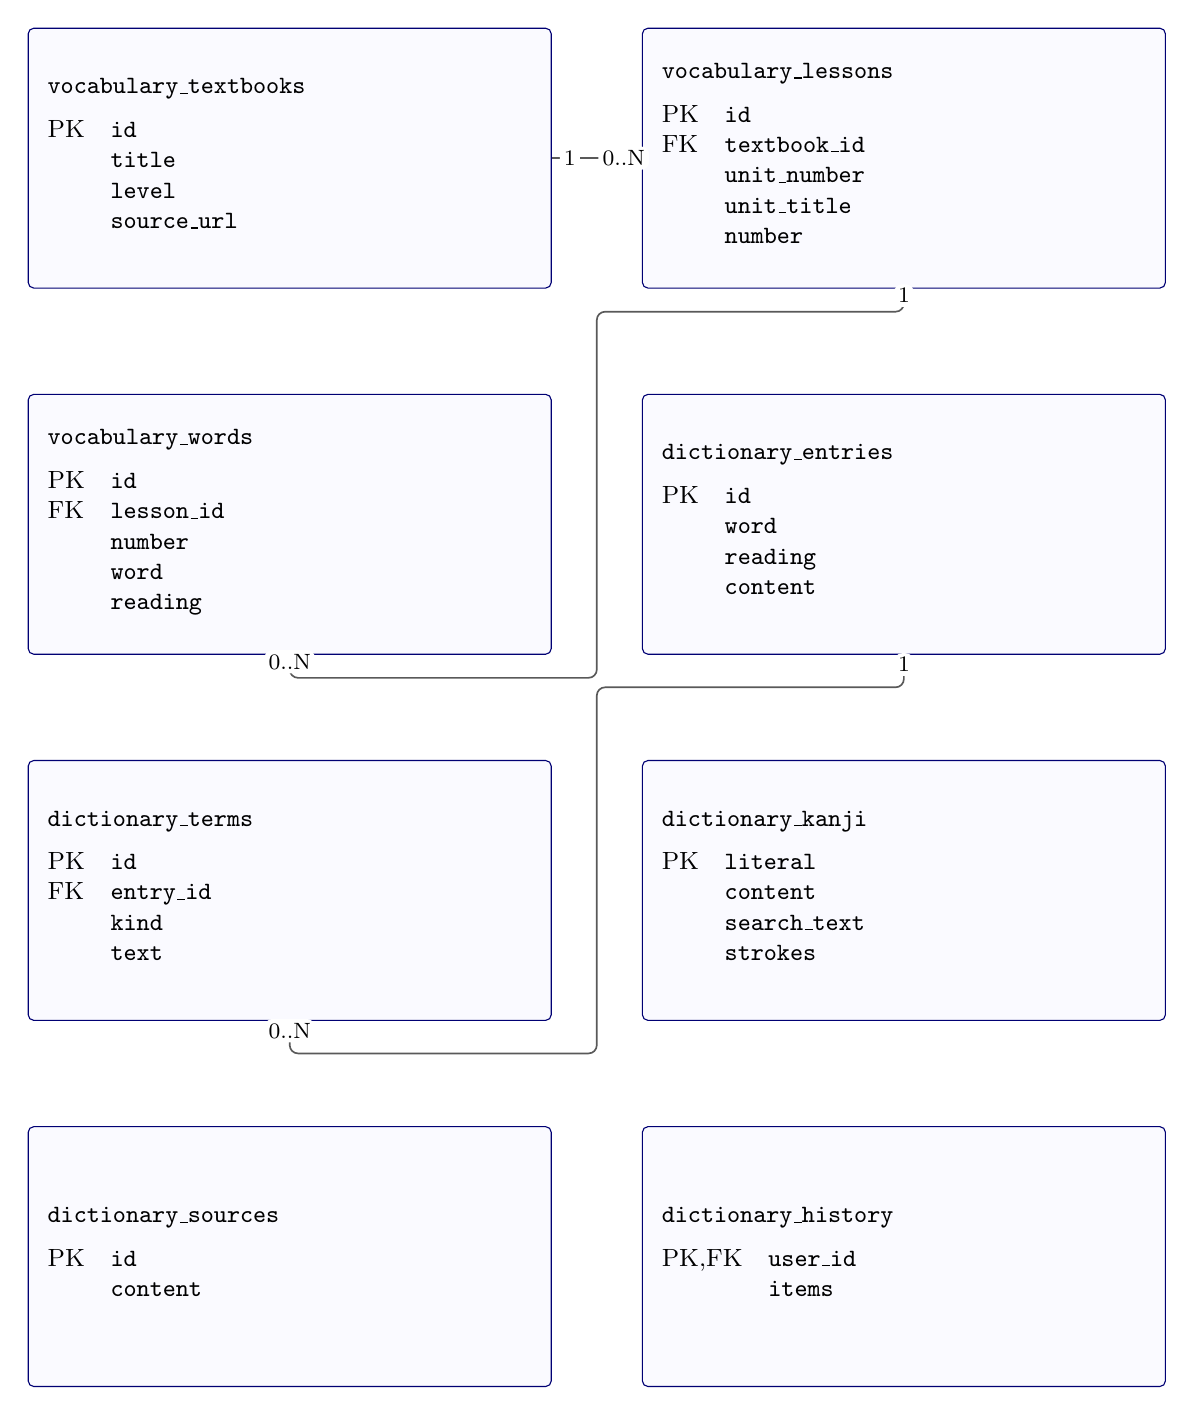
\begin{tikzpicture}[
entity/.style={draw=blue!45!black,rounded corners=2pt,fill=blue!2,inner sep=7pt,text width=6.15cm,minimum height=3.3cm,align=left,font=\fontsize{9}{11}\selectfont},
rel/.style={draw=black!65,line width=.6pt,rounded corners=3pt},
card/.style={fill=white,inner sep=1.5pt,font=\fontsize{8}{9}\selectfont}]
\node[entity] (vocabularytextbooks) at (-3.9,0) {\textbf{\texttt{vocabulary\_textbooks}}\\[5pt]\begin{tabular}{@{}l@{\quad}l@{}}PK & \texttt{id} \\
 & \texttt{title} \\
 & \texttt{level} \\
 & \texttt{source\_url} \\\end{tabular}};
\node[entity] (vocabularylessons) at (3.9,0) {\textbf{\texttt{vocabulary\_lessons}}\\[5pt]\begin{tabular}{@{}l@{\quad}l@{}}PK & \texttt{id} \\
FK & \texttt{textbook\_id} \\
 & \texttt{unit\_number} \\
 & \texttt{unit\_title} \\
 & \texttt{number} \\\end{tabular}};
\node[entity] (vocabularywords) at (-3.9,-4.65) {\textbf{\texttt{vocabulary\_words}}\\[5pt]\begin{tabular}{@{}l@{\quad}l@{}}PK & \texttt{id} \\
FK & \texttt{lesson\_id} \\
 & \texttt{number} \\
 & \texttt{word} \\
 & \texttt{reading} \\\end{tabular}};
\node[entity] (dictionaryentries) at (3.9,-4.65) {\textbf{\texttt{dictionary\_entries}}\\[5pt]\begin{tabular}{@{}l@{\quad}l@{}}PK & \texttt{id} \\
 & \texttt{word} \\
 & \texttt{reading} \\
 & \texttt{content} \\\end{tabular}};
\node[entity] (dictionaryterms) at (-3.9,-9.3) {\textbf{\texttt{dictionary\_terms}}\\[5pt]\begin{tabular}{@{}l@{\quad}l@{}}PK & \texttt{id} \\
FK & \texttt{entry\_id} \\
 & \texttt{kind} \\
 & \texttt{text} \\\end{tabular}};
\node[entity] (dictionarykanji) at (3.9,-9.3) {\textbf{\texttt{dictionary\_kanji}}\\[5pt]\begin{tabular}{@{}l@{\quad}l@{}}PK & \texttt{literal} \\
 & \texttt{content} \\
 & \texttt{search\_text} \\
 & \texttt{strokes} \\\end{tabular}};
\node[entity] (dictionarysources) at (-3.9,-13.950000000000001) {\textbf{\texttt{dictionary\_sources}}\\[5pt]\begin{tabular}{@{}l@{\quad}l@{}}PK & \texttt{id} \\
 & \texttt{content} \\\end{tabular}};
\node[entity] (dictionaryhistory) at (3.9,-13.950000000000001) {\textbf{\texttt{dictionary\_history}}\\[5pt]\begin{tabular}{@{}l@{\quad}l@{}}PK,FK & \texttt{user\_id} \\
 & \texttt{items} \\\end{tabular}};
\draw[rel] (vocabularylessons.west) -- node[card,pos=.2]{0..N} node[card,pos=.8]{1} (vocabularytextbooks.east);
\draw[rel] (vocabularywords.south) -- node[card,pos=.3]{0..N} (-3.9,-6.6000000000000005) -- (0,-6.6000000000000005) -- (0,-1.95) -- (3.9,-1.95) -- node[card,pos=.7]{1} (vocabularylessons.south);
\draw[rel] (dictionaryterms.south) -- node[card,pos=.3]{0..N} (-3.9,-11.37) -- (0,-11.37) -- (0,-6.720000000000001) -- (3.9,-6.720000000000001) -- node[card,pos=.7]{1} (dictionaryentries.south);
\end{tikzpicture}
\endgroup

  \caption{ERD: Vocabulary and Dictionary}
  \label{fig:erd-content}
\end{figure}
\clearpage
\subsection{Reading and Writing}
\begin{figure}[htbp]
  \centering
  \begingroup
\setstretch{1}
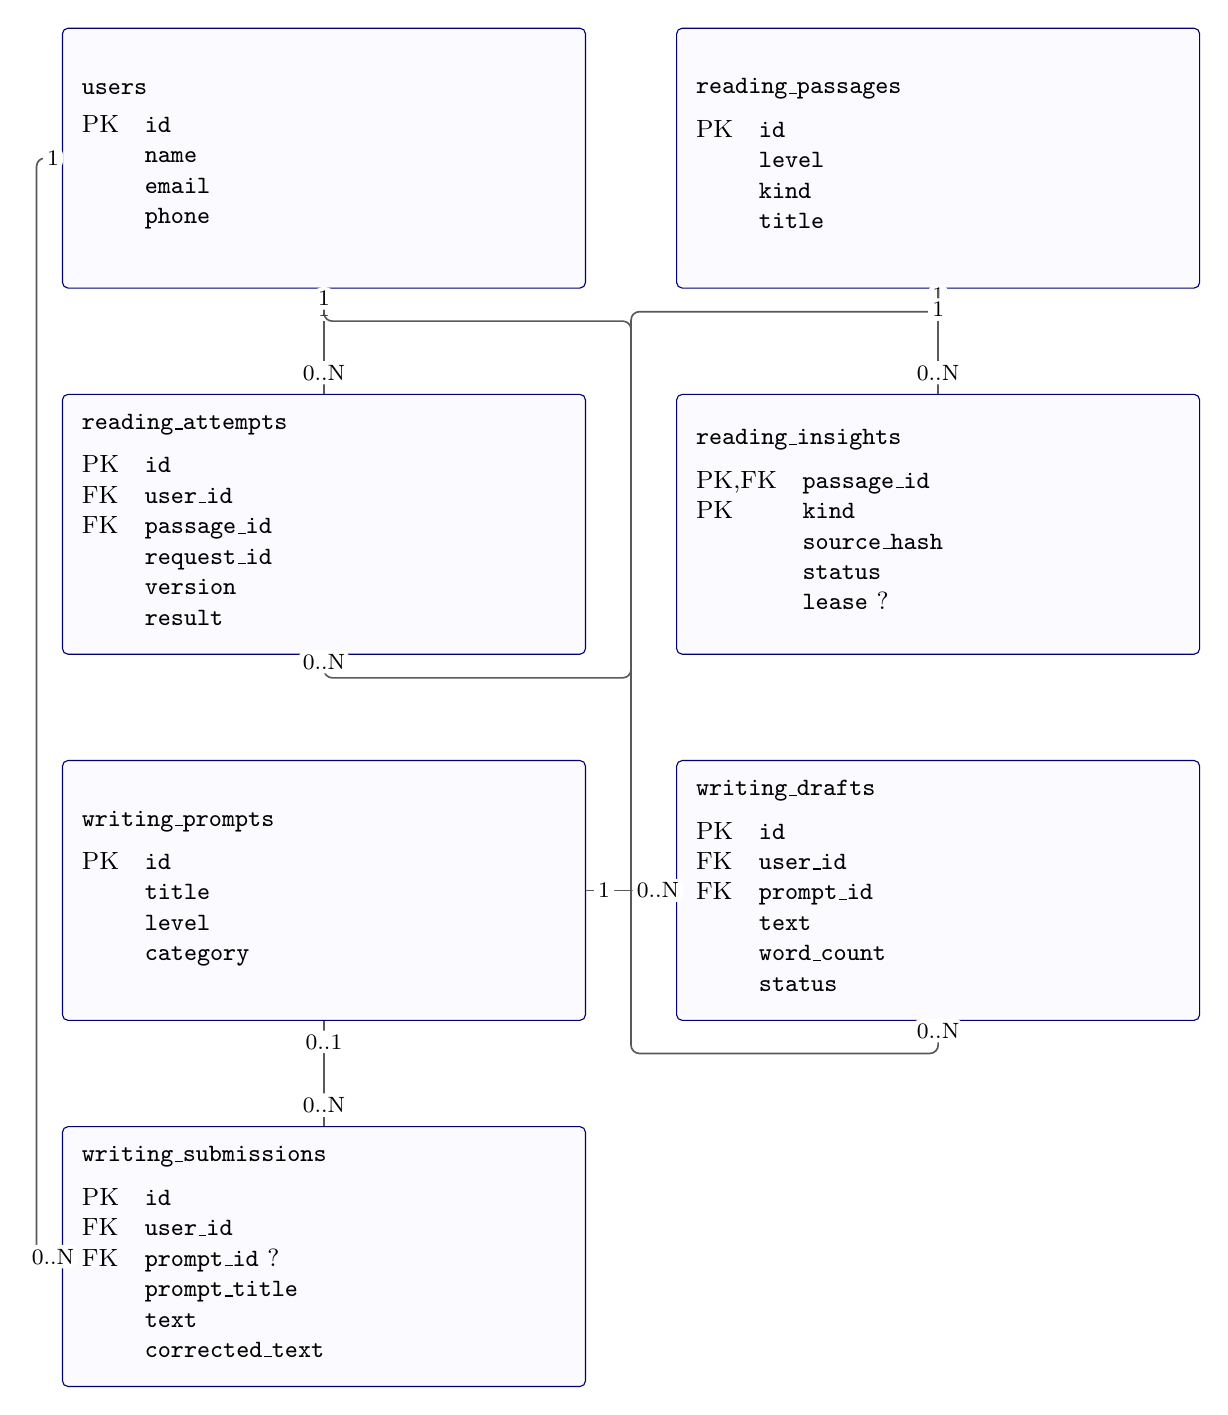
\begin{tikzpicture}[
entity/.style={draw=blue!45!black,rounded corners=2pt,fill=blue!2,inner sep=7pt,text width=6.15cm,minimum height=3.3cm,align=left,font=\fontsize{9}{11}\selectfont},
rel/.style={draw=black!65,line width=.6pt,rounded corners=3pt},
card/.style={fill=white,inner sep=1.5pt,font=\fontsize{8}{9}\selectfont}]
\node[entity] (users) at (-3.9,0) {\textbf{\texttt{users}}\\[5pt]\begin{tabular}{@{}l@{\quad}l@{}}PK & \texttt{id} \\
 & \texttt{name} \\
 & \texttt{email} \\
 & \texttt{phone} \\\end{tabular}};
\node[entity] (readingpassages) at (3.9,0) {\textbf{\texttt{reading\_passages}}\\[5pt]\begin{tabular}{@{}l@{\quad}l@{}}PK & \texttt{id} \\
 & \texttt{level} \\
 & \texttt{kind} \\
 & \texttt{title} \\\end{tabular}};
\node[entity] (readingattempts) at (-3.9,-4.65) {\textbf{\texttt{reading\_attempts}}\\[5pt]\begin{tabular}{@{}l@{\quad}l@{}}PK & \texttt{id} \\
FK & \texttt{user\_id} \\
FK & \texttt{passage\_id} \\
 & \texttt{request\_id} \\
 & \texttt{version} \\
 & \texttt{result} \\\end{tabular}};
\node[entity] (readinginsights) at (3.9,-4.65) {\textbf{\texttt{reading\_insights}}\\[5pt]\begin{tabular}{@{}l@{\quad}l@{}}PK,FK & \texttt{passage\_id} \\
PK & \texttt{kind} \\
 & \texttt{source\_hash} \\
 & \texttt{status} \\
 & \texttt{lease} ? \\\end{tabular}};
\node[entity] (writingprompts) at (-3.9,-9.3) {\textbf{\texttt{writing\_prompts}}\\[5pt]\begin{tabular}{@{}l@{\quad}l@{}}PK & \texttt{id} \\
 & \texttt{title} \\
 & \texttt{level} \\
 & \texttt{category} \\\end{tabular}};
\node[entity] (writingdrafts) at (3.9,-9.3) {\textbf{\texttt{writing\_drafts}}\\[5pt]\begin{tabular}{@{}l@{\quad}l@{}}PK & \texttt{id} \\
FK & \texttt{user\_id} \\
FK & \texttt{prompt\_id} \\
 & \texttt{text} \\
 & \texttt{word\_count} \\
 & \texttt{status} \\\end{tabular}};
\node[entity] (writingsubmissions) at (-3.9,-13.950000000000001) {\textbf{\texttt{writing\_submissions}}\\[5pt]\begin{tabular}{@{}l@{\quad}l@{}}PK & \texttt{id} \\
FK & \texttt{user\_id} \\
FK & \texttt{prompt\_id} ? \\
 & \texttt{prompt\_title} \\
 & \texttt{text} \\
 & \texttt{corrected\_text} \\\end{tabular}};
\draw[rel] (readingattempts.north) -- node[card,pos=.2]{0..N} node[card,pos=.8]{1} (users.south);
\draw[rel] (readingattempts.south) -- node[card,pos=.3]{0..N} (-3.9,-6.6000000000000005) -- (0,-6.6000000000000005) -- (0,-1.95) -- (3.9,-1.95) -- node[card,pos=.7]{1} (readingpassages.south);
\draw[rel] (readinginsights.north) -- node[card,pos=.2]{0..N} node[card,pos=.8]{1} (readingpassages.south);
\draw[rel] (writingdrafts.south) -- node[card,pos=.3]{0..N} (3.9,-11.37) -- (0,-11.37) -- (0,-2.07) -- (-3.9,-2.07) -- node[card,pos=.7]{1} (users.south);
\draw[rel] (writingdrafts.west) -- node[card,pos=.2]{0..N} node[card,pos=.8]{1} (writingprompts.east);
\draw[rel] (writingsubmissions.north) -- node[card,pos=.2]{0..N} node[card,pos=.8]{0..1} (writingprompts.south);
\draw[rel] (writingsubmissions.west) -- node[card,pos=.35]{0..N} (-7.55,-13.950000000000001) -- (-7.55,0) -- node[card,pos=.65]{1} (users.west);
\end{tikzpicture}
\endgroup

  \caption{ERD: Reading and Writing}
  \label{fig:erd-practice}
\end{figure}
\clearpage
\subsection{Scenarios and Conversation Sessions}
{\small\raggedright FK ghép: \texttt{(scenario\_id, scenario\_role\_id)} của \texttt{conversation\_sessions} tham chiếu \texttt{scenario\_roles.(scenario\_id, id)}. Quan hệ tự tham chiếu thể hiện phiên luyện tập lại.\par}

\begin{figure}[htbp]
  \centering
  \begingroup
\setstretch{1}
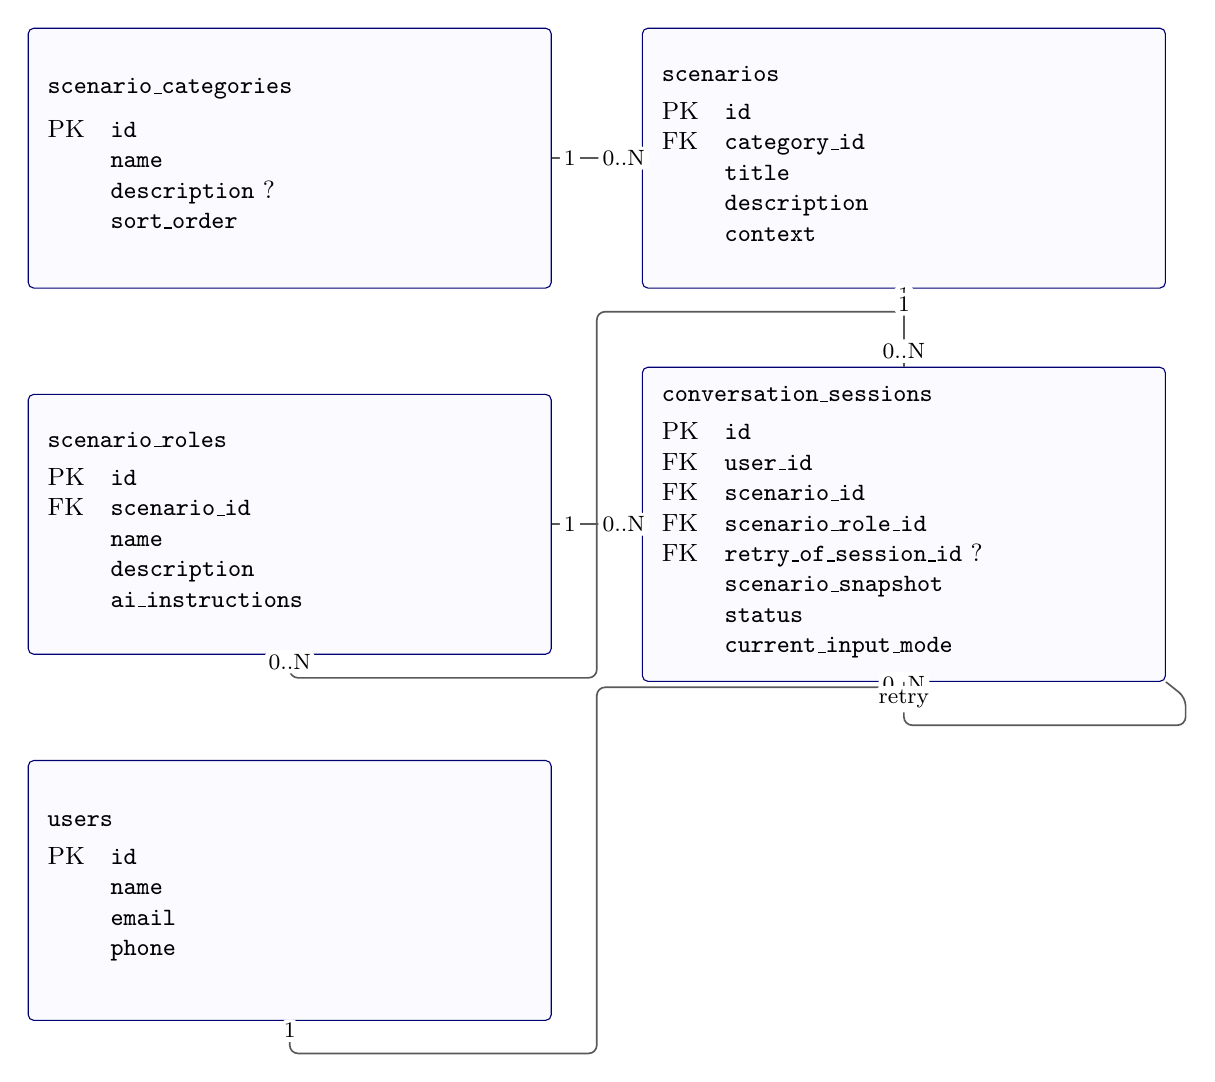
\begin{tikzpicture}[
entity/.style={draw=blue!45!black,rounded corners=2pt,fill=blue!2,inner sep=7pt,text width=6.15cm,minimum height=3.3cm,align=left,font=\fontsize{9}{11}\selectfont},
rel/.style={draw=black!65,line width=.6pt,rounded corners=3pt},
card/.style={fill=white,inner sep=1.5pt,font=\fontsize{8}{9}\selectfont}]
\node[entity] (scenariocategories) at (-3.9,0) {\textbf{\texttt{scenario\_categories}}\\[5pt]\begin{tabular}{@{}l@{\quad}l@{}}PK & \texttt{id} \\
 & \texttt{name} \\
 & \texttt{description} ? \\
 & \texttt{sort\_order} \\\end{tabular}};
\node[entity] (scenarios) at (3.9,0) {\textbf{\texttt{scenarios}}\\[5pt]\begin{tabular}{@{}l@{\quad}l@{}}PK & \texttt{id} \\
FK & \texttt{category\_id} \\
 & \texttt{title} \\
 & \texttt{description} \\
 & \texttt{context} \\\end{tabular}};
\node[entity] (scenarioroles) at (-3.9,-4.65) {\textbf{\texttt{scenario\_roles}}\\[5pt]\begin{tabular}{@{}l@{\quad}l@{}}PK & \texttt{id} \\
FK & \texttt{scenario\_id} \\
 & \texttt{name} \\
 & \texttt{description} \\
 & \texttt{ai\_instructions} \\\end{tabular}};
\node[entity] (conversationsessions) at (3.9,-4.65) {\textbf{\texttt{conversation\_sessions}}\\[5pt]\begin{tabular}{@{}l@{\quad}l@{}}PK & \texttt{id} \\
FK & \texttt{user\_id} \\
FK & \texttt{scenario\_id} \\
FK & \texttt{scenario\_role\_id} \\
FK & \texttt{retry\_of\_session\_id} ? \\
 & \texttt{scenario\_snapshot} \\
 & \texttt{status} \\
 & \texttt{current\_input\_mode} \\\end{tabular}};
\node[entity] (users) at (-3.9,-9.3) {\textbf{\texttt{users}}\\[5pt]\begin{tabular}{@{}l@{\quad}l@{}}PK & \texttt{id} \\
 & \texttt{name} \\
 & \texttt{email} \\
 & \texttt{phone} \\\end{tabular}};
\draw[rel] (scenarios.west) -- node[card,pos=.2]{0..N} node[card,pos=.8]{1} (scenariocategories.east);
\draw[rel] (scenarioroles.south) -- node[card,pos=.3]{0..N} (-3.9,-6.6000000000000005) -- (0,-6.6000000000000005) -- (0,-1.95) -- (3.9,-1.95) -- node[card,pos=.7]{1} (scenarios.south);
\draw[rel] (conversationsessions.south) -- node[card,pos=.3]{0..N} (3.9,-6.720000000000001) -- (0,-6.720000000000001) -- (0,-11.37) -- (-3.9,-11.37) -- node[card,pos=.7]{1} (users.south);
\draw[rel] (conversationsessions.north) -- node[card,pos=.2]{0..N} node[card,pos=.8]{1} (scenarios.south);
\draw[rel] (conversationsessions.west) -- node[card,pos=.2]{0..N} node[card,pos=.8]{1} (scenarioroles.east);
\draw[rel] (conversationsessions.south east) -- ++(.25,-.2) -- ++(0,-.35) -| (conversationsessions.south) node[card,pos=.8]{retry};
\end{tikzpicture}
\endgroup

  \caption{ERD: Scenarios and Conversation Sessions}
  \label{fig:erd-scenarios}
\end{figure}
\clearpage
\subsection{Conversation Records and Evaluation}
{\small\raggedright FK ghép: \texttt{conversation\_audio\_assets.(session\_id, message\_id)} tham chiếu \texttt{conversation\_messages.(session\_id, id)}. \texttt{storage\_key} lưu định danh tệp, không lưu nội dung âm thanh. Các FK của \texttt{conversation\_sessions} đến users/scenarios được thể hiện ở hình trước.\par}

\begin{figure}[htbp]
  \centering
  \begingroup
\setstretch{1}
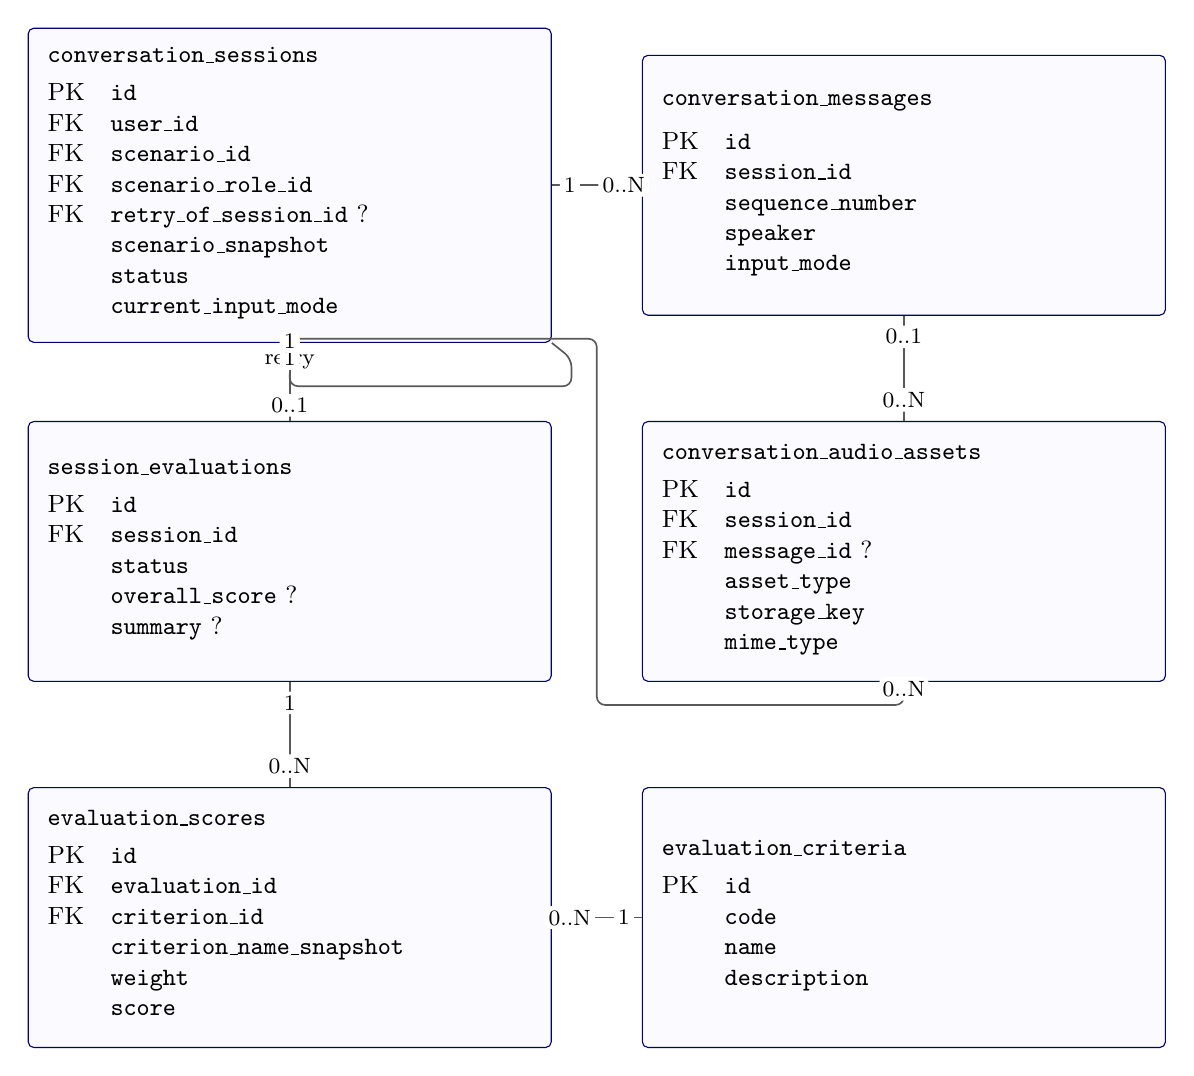
\begin{tikzpicture}[
entity/.style={draw=blue!45!black,rounded corners=2pt,fill=blue!2,inner sep=7pt,text width=6.15cm,minimum height=3.3cm,align=left,font=\fontsize{9}{11}\selectfont},
rel/.style={draw=black!65,line width=.6pt,rounded corners=3pt},
card/.style={fill=white,inner sep=1.5pt,font=\fontsize{8}{9}\selectfont}]
\node[entity] (conversationsessions) at (-3.9,0) {\textbf{\texttt{conversation\_sessions}}\\[5pt]\begin{tabular}{@{}l@{\quad}l@{}}PK & \texttt{id} \\
FK & \texttt{user\_id} \\
FK & \texttt{scenario\_id} \\
FK & \texttt{scenario\_role\_id} \\
FK & \texttt{retry\_of\_session\_id} ? \\
 & \texttt{scenario\_snapshot} \\
 & \texttt{status} \\
 & \texttt{current\_input\_mode} \\\end{tabular}};
\node[entity] (conversationmessages) at (3.9,0) {\textbf{\texttt{conversation\_messages}}\\[5pt]\begin{tabular}{@{}l@{\quad}l@{}}PK & \texttt{id} \\
FK & \texttt{session\_id} \\
 & \texttt{sequence\_number} \\
 & \texttt{speaker} \\
 & \texttt{input\_mode} \\\end{tabular}};
\node[entity] (sessionevaluations) at (-3.9,-4.65) {\textbf{\texttt{session\_evaluations}}\\[5pt]\begin{tabular}{@{}l@{\quad}l@{}}PK & \texttt{id} \\
FK & \texttt{session\_id} \\
 & \texttt{status} \\
 & \texttt{overall\_score} ? \\
 & \texttt{summary} ? \\\end{tabular}};
\node[entity] (conversationaudioassets) at (3.9,-4.65) {\textbf{\texttt{conversation\_audio\_assets}}\\[5pt]\begin{tabular}{@{}l@{\quad}l@{}}PK & \texttt{id} \\
FK & \texttt{session\_id} \\
FK & \texttt{message\_id} ? \\
 & \texttt{asset\_type} \\
 & \texttt{storage\_key} \\
 & \texttt{mime\_type} \\\end{tabular}};
\node[entity] (evaluationscores) at (-3.9,-9.3) {\textbf{\texttt{evaluation\_scores}}\\[5pt]\begin{tabular}{@{}l@{\quad}l@{}}PK & \texttt{id} \\
FK & \texttt{evaluation\_id} \\
FK & \texttt{criterion\_id} \\
 & \texttt{criterion\_name\_snapshot} \\
 & \texttt{weight} \\
 & \texttt{score} \\\end{tabular}};
\node[entity] (evaluationcriteria) at (3.9,-9.3) {\textbf{\texttt{evaluation\_criteria}}\\[5pt]\begin{tabular}{@{}l@{\quad}l@{}}PK & \texttt{id} \\
 & \texttt{code} \\
 & \texttt{name} \\
 & \texttt{description} \\\end{tabular}};
\draw[rel] (conversationsessions.south east) -- ++(.25,-.2) -- ++(0,-.35) -| (conversationsessions.south) node[card,pos=.8]{retry};
\draw[rel] (conversationmessages.west) -- node[card,pos=.2]{0..N} node[card,pos=.8]{1} (conversationsessions.east);
\draw[rel] (sessionevaluations.north) -- node[card,pos=.2]{0..1} node[card,pos=.8]{1} (conversationsessions.south);
\draw[rel] (conversationaudioassets.north) -- node[card,pos=.2]{0..N} node[card,pos=.8]{0..1} (conversationmessages.south);
\draw[rel] (conversationaudioassets.south) -- node[card,pos=.3]{0..N} (3.9,-6.6000000000000005) -- (0,-6.6000000000000005) -- (0,-1.95) -- (-3.9,-1.95) -- node[card,pos=.7]{1} (conversationsessions.south);
\draw[rel] (evaluationscores.east) -- node[card,pos=.2]{0..N} node[card,pos=.8]{1} (evaluationcriteria.west);
\draw[rel] (evaluationscores.north) -- node[card,pos=.2]{0..N} node[card,pos=.8]{1} (sessionevaluations.south);
\end{tikzpicture}
\endgroup

  \caption{ERD: Conversation Records and Evaluation}
  \label{fig:erd-evaluation}
\end{figure}
\clearpage
\subsection{Rooms and Matchmaking}
{\small\raggedright Các trường \texttt{created\_by}, \texttt{invited\_by} và \texttt{invitee\_user\_id} đều tham chiếu users. \texttt{room\_members} hiện thực quan hệ N--N giữa users và rooms.\par}

\begin{figure}[htbp]
  \centering
  \begingroup
\setstretch{1}
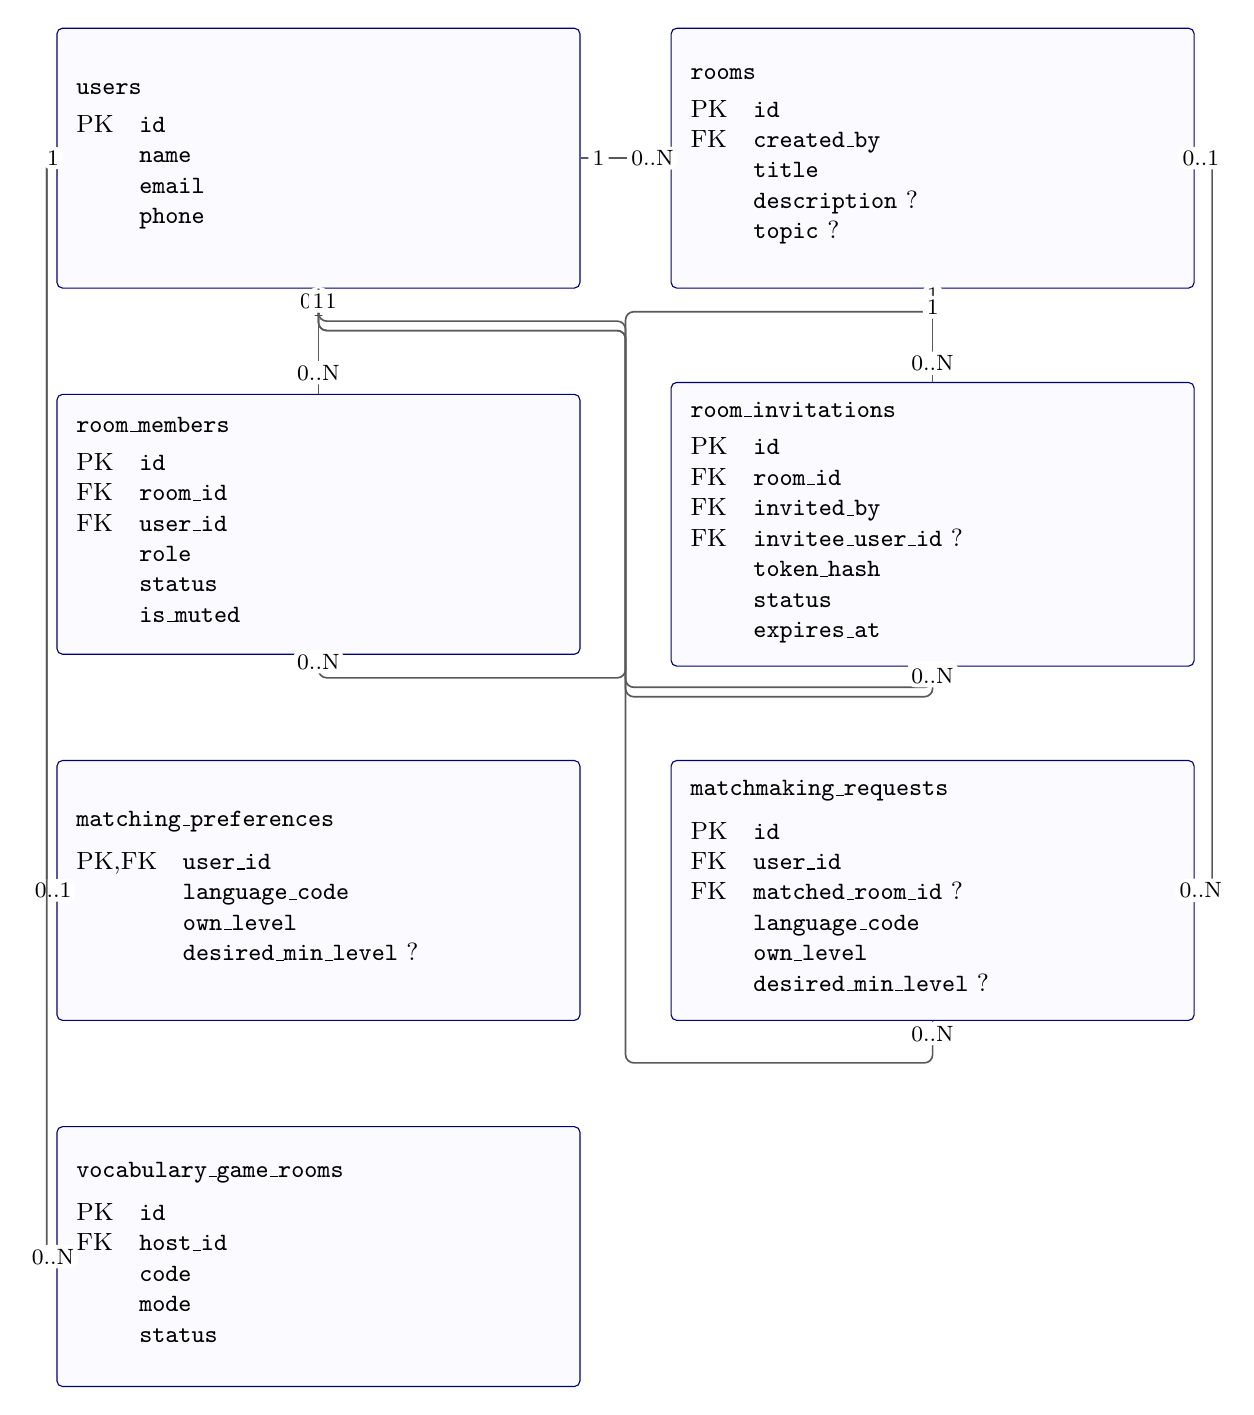
\begin{tikzpicture}[
entity/.style={draw=blue!45!black,rounded corners=2pt,fill=blue!2,inner sep=7pt,text width=6.15cm,minimum height=3.3cm,align=left,font=\fontsize{9}{11}\selectfont},
rel/.style={draw=black!65,line width=.6pt,rounded corners=3pt},
card/.style={fill=white,inner sep=1.5pt,font=\fontsize{8}{9}\selectfont}]
\node[entity] (users) at (-3.9,0) {\textbf{\texttt{users}}\\[5pt]\begin{tabular}{@{}l@{\quad}l@{}}PK & \texttt{id} \\
 & \texttt{name} \\
 & \texttt{email} \\
 & \texttt{phone} \\\end{tabular}};
\node[entity] (rooms) at (3.9,0) {\textbf{\texttt{rooms}}\\[5pt]\begin{tabular}{@{}l@{\quad}l@{}}PK & \texttt{id} \\
FK & \texttt{created\_by} \\
 & \texttt{title} \\
 & \texttt{description} ? \\
 & \texttt{topic} ? \\\end{tabular}};
\node[entity] (roommembers) at (-3.9,-4.65) {\textbf{\texttt{room\_members}}\\[5pt]\begin{tabular}{@{}l@{\quad}l@{}}PK & \texttt{id} \\
FK & \texttt{room\_id} \\
FK & \texttt{user\_id} \\
 & \texttt{role} \\
 & \texttt{status} \\
 & \texttt{is\_muted} \\\end{tabular}};
\node[entity] (roominvitations) at (3.9,-4.65) {\textbf{\texttt{room\_invitations}}\\[5pt]\begin{tabular}{@{}l@{\quad}l@{}}PK & \texttt{id} \\
FK & \texttt{room\_id} \\
FK & \texttt{invited\_by} \\
FK & \texttt{invitee\_user\_id} ? \\
 & \texttt{token\_hash} \\
 & \texttt{status} \\
 & \texttt{expires\_at} \\\end{tabular}};
\node[entity] (matchingpreferences) at (-3.9,-9.3) {\textbf{\texttt{matching\_preferences}}\\[5pt]\begin{tabular}{@{}l@{\quad}l@{}}PK,FK & \texttt{user\_id} \\
 & \texttt{language\_code} \\
 & \texttt{own\_level} \\
 & \texttt{desired\_min\_level} ? \\\end{tabular}};
\node[entity] (matchmakingrequests) at (3.9,-9.3) {\textbf{\texttt{matchmaking\_requests}}\\[5pt]\begin{tabular}{@{}l@{\quad}l@{}}PK & \texttt{id} \\
FK & \texttt{user\_id} \\
FK & \texttt{matched\_room\_id} ? \\
 & \texttt{language\_code} \\
 & \texttt{own\_level} \\
 & \texttt{desired\_min\_level} ? \\\end{tabular}};
\node[entity] (vocabularygamerooms) at (-3.9,-13.950000000000001) {\textbf{\texttt{vocabulary\_game\_rooms}}\\[5pt]\begin{tabular}{@{}l@{\quad}l@{}}PK & \texttt{id} \\
FK & \texttt{host\_id} \\
 & \texttt{code} \\
 & \texttt{mode} \\
 & \texttt{status} \\\end{tabular}};
\draw[rel] (rooms.west) -- node[card,pos=.2]{0..N} node[card,pos=.8]{1} (users.east);
\draw[rel] (roommembers.south) -- node[card,pos=.3]{0..N} (-3.9,-6.6000000000000005) -- (0,-6.6000000000000005) -- (0,-1.95) -- (3.9,-1.95) -- node[card,pos=.7]{1} (rooms.south);
\draw[rel] (roommembers.north) -- node[card,pos=.2]{0..N} node[card,pos=.8]{1} (users.south);
\draw[rel] (roominvitations.south) -- node[card,pos=.3]{0..N} (3.9,-6.720000000000001) -- (0,-6.720000000000001) -- (0,-2.07) -- (-3.9,-2.07) -- node[card,pos=.7]{1} (users.south);
\draw[rel] (roominvitations.south) -- node[card,pos=.3]{0..N} (3.9,-6.840000000000001) -- (0,-6.840000000000001) -- (0,-2.19) -- (-3.9,-2.19) -- node[card,pos=.7]{0..1} (users.south);
\draw[rel] (roominvitations.north) -- node[card,pos=.2]{0..N} node[card,pos=.8]{1} (rooms.south);
\draw[rel] (matchingpreferences.west) -- node[card,pos=.35]{0..1} (-7.35,-9.3) -- (-7.35,0) -- node[card,pos=.65]{1} (users.west);
\draw[rel] (matchmakingrequests.east) -- node[card,pos=.35]{0..N} (7.449999999999999,-9.3) -- (7.449999999999999,0) -- node[card,pos=.65]{0..1} (rooms.east);
\draw[rel] (matchmakingrequests.south) -- node[card,pos=.3]{0..N} (3.9,-11.49) -- (0,-11.49) -- (0,-2.19) -- (-3.9,-2.19) -- node[card,pos=.7]{1} (users.south);
\draw[rel] (vocabularygamerooms.west) -- node[card,pos=.35]{0..N} (-7.35,-13.950000000000001) -- (-7.35,0) -- node[card,pos=.65]{1} (users.west);
\end{tikzpicture}
\endgroup

  \caption{ERD: Rooms and Matchmaking}
  \label{fig:erd-rooms}
\end{figure}
\clearpage
\subsection{Shadowing and Video Examples}
{\small\raggedright Hai cụm Shadowing và video ví dụ độc lập ở mức FK; \texttt{shadowing\_jobs.video\_id} không có FK tới \texttt{example\_videos}. Bảng nối \texttt{shadowing\_requests} hiện thực quan hệ N--N giữa users và shadowing\_jobs.\par}

\begin{figure}[htbp]
  \centering
  \begingroup
\setstretch{1}
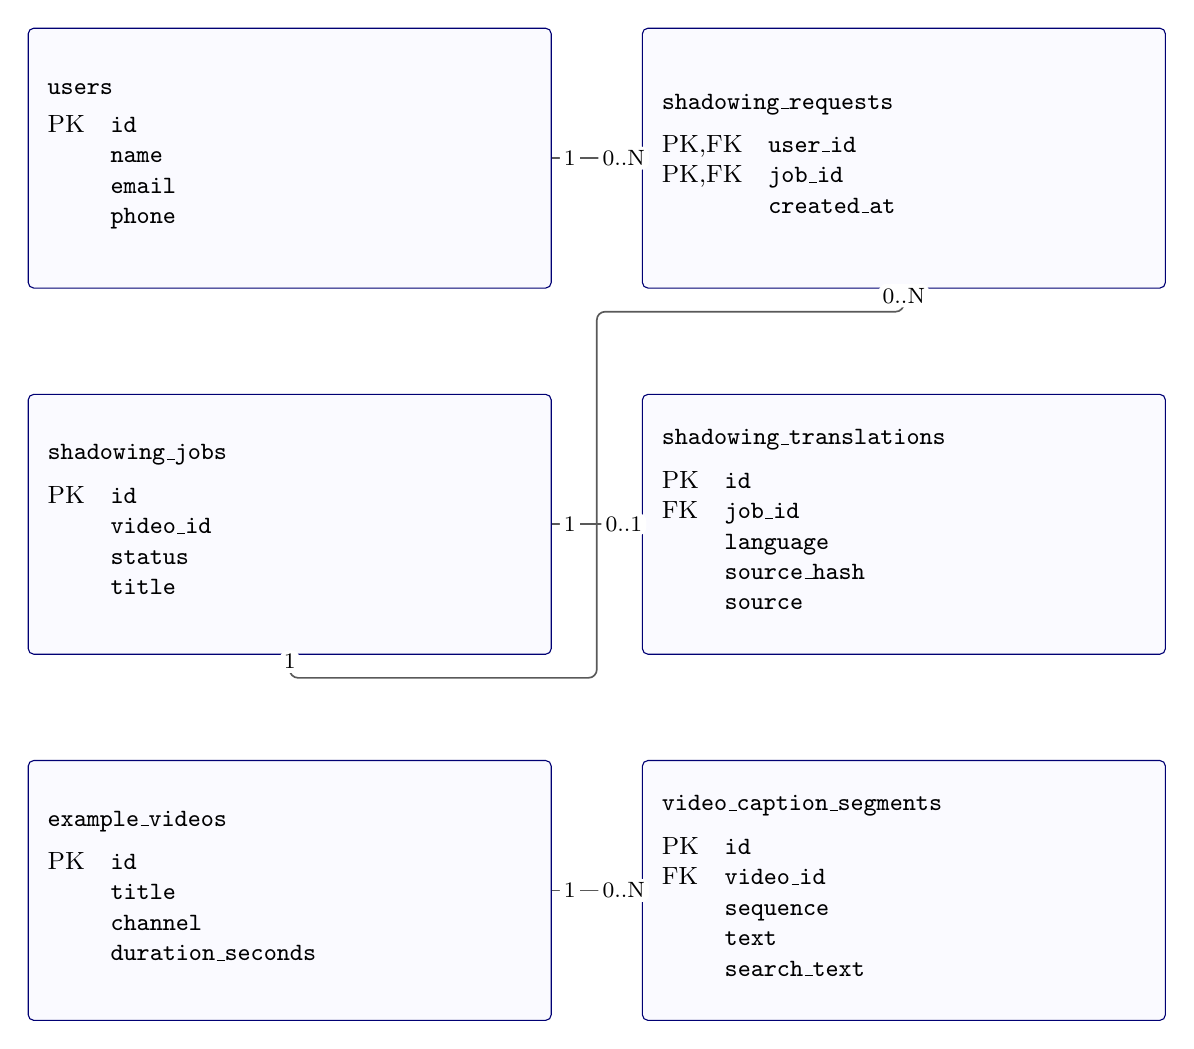
\begin{tikzpicture}[
entity/.style={draw=blue!45!black,rounded corners=2pt,fill=blue!2,inner sep=7pt,text width=6.15cm,minimum height=3.3cm,align=left,font=\fontsize{9}{11}\selectfont},
rel/.style={draw=black!65,line width=.6pt,rounded corners=3pt},
card/.style={fill=white,inner sep=1.5pt,font=\fontsize{8}{9}\selectfont}]
\node[entity] (users) at (-3.9,0) {\textbf{\texttt{users}}\\[5pt]\begin{tabular}{@{}l@{\quad}l@{}}PK & \texttt{id} \\
 & \texttt{name} \\
 & \texttt{email} \\
 & \texttt{phone} \\\end{tabular}};
\node[entity] (shadowingrequests) at (3.9,0) {\textbf{\texttt{shadowing\_requests}}\\[5pt]\begin{tabular}{@{}l@{\quad}l@{}}PK,FK & \texttt{user\_id} \\
PK,FK & \texttt{job\_id} \\
 & \texttt{created\_at} \\\end{tabular}};
\node[entity] (shadowingjobs) at (-3.9,-4.65) {\textbf{\texttt{shadowing\_jobs}}\\[5pt]\begin{tabular}{@{}l@{\quad}l@{}}PK & \texttt{id} \\
 & \texttt{video\_id} \\
 & \texttt{status} \\
 & \texttt{title} \\\end{tabular}};
\node[entity] (shadowingtranslations) at (3.9,-4.65) {\textbf{\texttt{shadowing\_translations}}\\[5pt]\begin{tabular}{@{}l@{\quad}l@{}}PK & \texttt{id} \\
FK & \texttt{job\_id} \\
 & \texttt{language} \\
 & \texttt{source\_hash} \\
 & \texttt{source} \\\end{tabular}};
\node[entity] (examplevideos) at (-3.9,-9.3) {\textbf{\texttt{example\_videos}}\\[5pt]\begin{tabular}{@{}l@{\quad}l@{}}PK & \texttt{id} \\
 & \texttt{title} \\
 & \texttt{channel} \\
 & \texttt{duration\_seconds} \\\end{tabular}};
\node[entity] (videocaptionsegments) at (3.9,-9.3) {\textbf{\texttt{video\_caption\_segments}}\\[5pt]\begin{tabular}{@{}l@{\quad}l@{}}PK & \texttt{id} \\
FK & \texttt{video\_id} \\
 & \texttt{sequence} \\
 & \texttt{text} \\
 & \texttt{search\_text} \\\end{tabular}};
\draw[rel] (shadowingrequests.west) -- node[card,pos=.2]{0..N} node[card,pos=.8]{1} (users.east);
\draw[rel] (shadowingrequests.south) -- node[card,pos=.3]{0..N} (3.9,-1.95) -- (0,-1.95) -- (0,-6.6000000000000005) -- (-3.9,-6.6000000000000005) -- node[card,pos=.7]{1} (shadowingjobs.south);
\draw[rel] (shadowingtranslations.west) -- node[card,pos=.2]{0..1} node[card,pos=.8]{1} (shadowingjobs.east);
\draw[rel] (videocaptionsegments.west) -- node[card,pos=.2]{0..N} node[card,pos=.8]{1} (examplevideos.east);
\end{tikzpicture}
\endgroup

  \caption{ERD: Shadowing and Video Examples}
  \label{fig:erd-shadowing}
\end{figure}
\clearpage
\subsection{Beta Quotas and AI Usage}
{\small\raggedright Các bảng beta phản ánh schema hiện có, không khẳng định mọi tính năng beta đều đang được bật.\par}

\begin{figure}[htbp]
  \centering
  \begingroup
\setstretch{1}
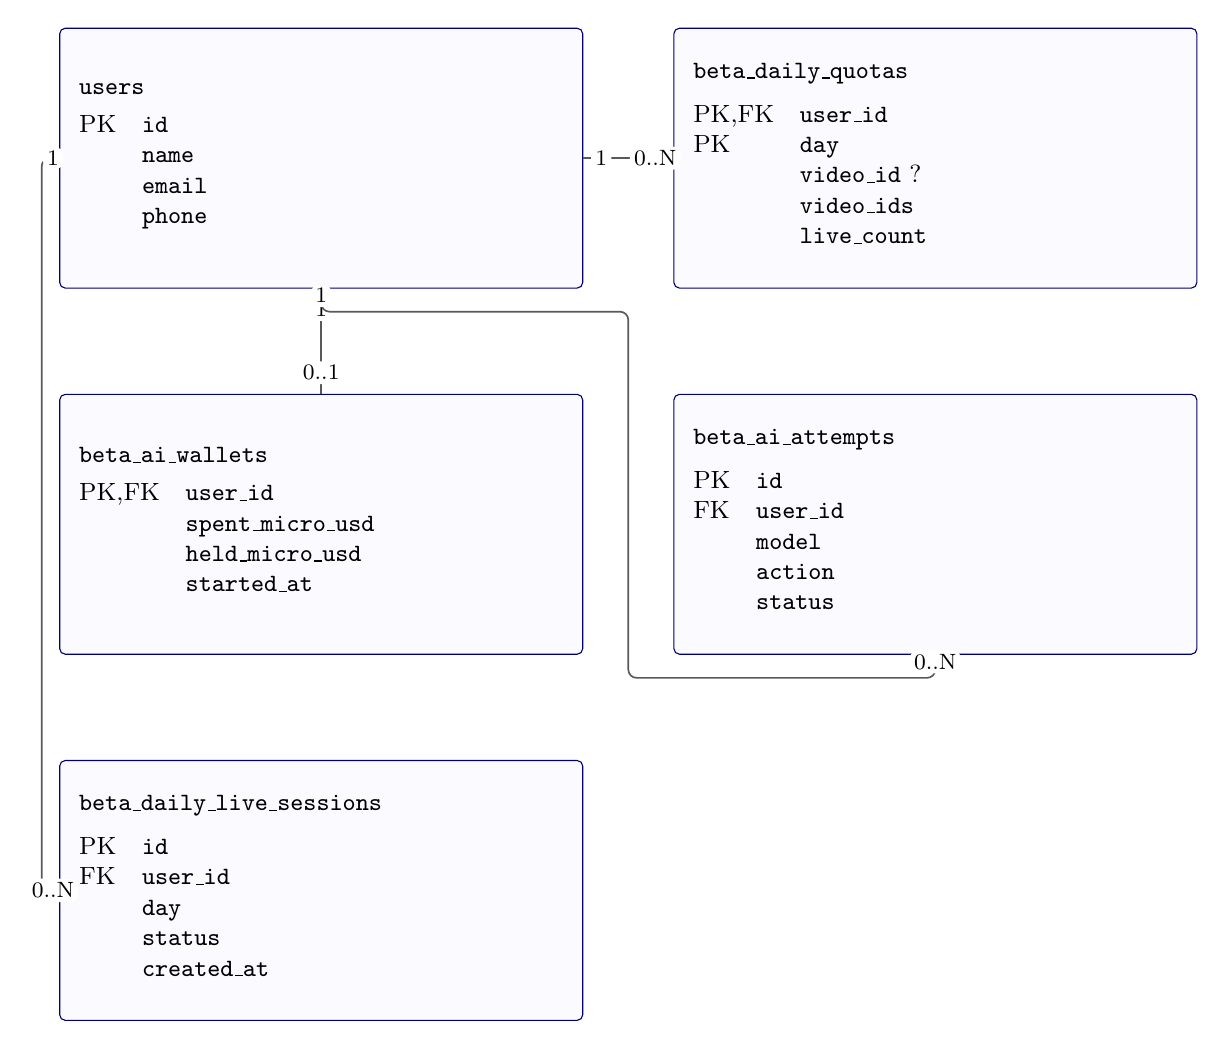
\begin{tikzpicture}[
entity/.style={draw=blue!45!black,rounded corners=2pt,fill=blue!2,inner sep=7pt,text width=6.15cm,minimum height=3.3cm,align=left,font=\fontsize{9}{11}\selectfont},
rel/.style={draw=black!65,line width=.6pt,rounded corners=3pt},
card/.style={fill=white,inner sep=1.5pt,font=\fontsize{8}{9}\selectfont}]
\node[entity] (users) at (-3.9,0) {\textbf{\texttt{users}}\\[5pt]\begin{tabular}{@{}l@{\quad}l@{}}PK & \texttt{id} \\
 & \texttt{name} \\
 & \texttt{email} \\
 & \texttt{phone} \\\end{tabular}};
\node[entity] (betadailyquotas) at (3.9,0) {\textbf{\texttt{beta\_daily\_quotas}}\\[5pt]\begin{tabular}{@{}l@{\quad}l@{}}PK,FK & \texttt{user\_id} \\
PK & \texttt{day} \\
 & \texttt{video\_id} ? \\
 & \texttt{video\_ids} \\
 & \texttt{live\_count} \\\end{tabular}};
\node[entity] (betaaiwallets) at (-3.9,-4.65) {\textbf{\texttt{beta\_ai\_wallets}}\\[5pt]\begin{tabular}{@{}l@{\quad}l@{}}PK,FK & \texttt{user\_id} \\
 & \texttt{spent\_micro\_usd} \\
 & \texttt{held\_micro\_usd} \\
 & \texttt{started\_at} \\\end{tabular}};
\node[entity] (betaaiattempts) at (3.9,-4.65) {\textbf{\texttt{beta\_ai\_attempts}}\\[5pt]\begin{tabular}{@{}l@{\quad}l@{}}PK & \texttt{id} \\
FK & \texttt{user\_id} \\
 & \texttt{model} \\
 & \texttt{action} \\
 & \texttt{status} \\\end{tabular}};
\node[entity] (betadailylivesessions) at (-3.9,-9.3) {\textbf{\texttt{beta\_daily\_live\_sessions}}\\[5pt]\begin{tabular}{@{}l@{\quad}l@{}}PK & \texttt{id} \\
FK & \texttt{user\_id} \\
 & \texttt{day} \\
 & \texttt{status} \\
 & \texttt{created\_at} \\\end{tabular}};
\draw[rel] (betadailyquotas.west) -- node[card,pos=.2]{0..N} node[card,pos=.8]{1} (users.east);
\draw[rel] (betaaiwallets.north) -- node[card,pos=.2]{0..1} node[card,pos=.8]{1} (users.south);
\draw[rel] (betaaiattempts.south) -- node[card,pos=.3]{0..N} (3.9,-6.6000000000000005) -- (0,-6.6000000000000005) -- (0,-1.95) -- (-3.9,-1.95) -- node[card,pos=.7]{1} (users.south);
\draw[rel] (betadailylivesessions.west) -- node[card,pos=.35]{0..N} (-7.449999999999999,-9.3) -- (-7.449999999999999,0) -- node[card,pos=.65]{1} (users.west);
\end{tikzpicture}
\endgroup

  \caption{ERD: Beta Quotas and AI Usage}
  \label{fig:erd-beta}
\end{figure}
\clearpage
\section{FUNCTIONAL DESIGN}
\subsection{Use Case Diagram}
\subsection{Use Case Specification}
\subsection{Business Process Flow}
\section{UI/UX DESIGN}
\section{TECHNOLOGIES USED}

% ---- SAMPLE TABLE (delete when writing): caption ABOVE the table,
% ---- regular type, centred, numbered by chapter (QD 675, sec. 6).
\begin{table}[htbp]
  \caption{Technologies used in the system (sample)}
  \label{tab:tech-sample}
  \centering
  \begin{tabular}{@{}lll@{}}
    \toprule
    \textbf{Layer} & \textbf{Technology} & \textbf{Purpose} \\
    \midrule
    Frontend  & React.js & User interface \\
    Backend   & Python   & Business logic, LLM integration \\
    Cloud     & AWS      & Deployment and hosting \\
    \bottomrule
  \end{tabular}
\end{table}
\section{MVP DEVELOPMENT}
\subsection{Core Features}
\subsection{Trial Version}
\subsection{Outstanding Value of the Product}
\section{CHAPTER SUMMARY}
